% !Mode:: "TeX:UTF-8"
\documentclass[10pt,journal]{IEEEtran}
\usepackage{subfig}
\usepackage{graphicx}
\usepackage{amsmath}
\usepackage{algorithm}
\usepackage{algorithmic}
\usepackage{comment}
\usepackage{multirow}

\graphicspath{figures/}

\newtheorem{theorem}{Theorem}
\newtheorem{lemma}{Lemma}
\newtheorem{definition}{Definition}

\begin{document}
\title{Delay Analysis and Buffer Optimization for Priority-Aware Networks-on-Chip (NoC)}
%\onecolumn
%\author{\IEEEauthorblockN{Baoliang Li}}

\author{Baoliang~Li, %~\IEEEmembership{Student Member,~IEEE,}
        Zeljko Zilic, %~\IEEEmembership{Senior Member,~IEEE,}
        Wenhua~Dou, %~\IEEEmembership{Non-Member,~IEEE}% <-this % stops a space
\thanks{Baoliang~Li and Wenhua Dou are with the College of Computer Science, National University of Defense Technology, Changsha 410073, P.R. China}%
\thanks{Zeljko Zilic are with Department of Electrical \& Computer Engineering, McGill University, Montreal H3A-2A7, Quebec, Canada}%
\thanks{Manuscript received XX XX, 2014; revised XX XX, 2014.}}

\markboth{Journal of XXX,~Vol.~XX, No.~XX, XX~2014}%
{Li \MakeLowercase{\textit{et al.}}: A Delay and Backlog Model for Priority-Aware Networks-on-Chip (NoC)}

\maketitle

\begin{abstract}
Networks-on-Chip (NoC) is a key component for modern Chip-MultiProcessors(CMPs) and System-on-Chip (SoC). Among all the implementation alternatives, priority-aware wormhole-switched NoC is promising to meet the rigorous requirements of on-chip latency-aware communication, e.g. cache coherent protocol and multimedia applications. The end-to-end latency and buffer requirement analysis are very important for the development of real-time applications on this platform. In this paper, we first propose a Real-Time Calculus (RTC) based performance model for the priority-aware NoC. Then, we propose an end-to-end latency analysis algorithm and a buffer optimization algorithm. Our algorithms are topology-insensitive, it takes as input the scheduling network model and the application traffic characterization, and gives the end-to-end latency and buffer requirement for each traffic flow. Our model enables the fast performance evaluation and buffer optimization of priority-aware NoC, which can be used for application mapping, routing selection and power reduction. Experiment results demonstrate the effectiveness and tightness of our model. In addition, further comparisons with other theoretical models also indicates that, our method outperforms the existing methods while the tightness of the derived delay and backlog bound are considered.
\end{abstract}
\begin{IEEEkeywords}
Networks-on-Chip (NoC), priority-aware, wormhole switch, real-time calculus, delay and backlog bound
\end{IEEEkeywords}

\section{Introduction}
Conventional interconnection paradigms, e.g. bus, ring and point-to-point links, are not able to meet the strict and complex communication requirements of modern large scale Chip-MultiProcessors (CMPs) and System-on-Chip (SoC). As an alternative, Networks-on-Chip (NoC) is proposed to provide better scalability, higher power efficiency, and low-latency global communication, etc. As a key component of CMPs and SoC, NoC must be well designed to meet the rigorous requirements on end-to-end latency, buffer constraint, throughput and power, etc. Although various proposals have been emerged, with each focusing on improving different performance metrics of on-chip communication, most of the existing research on NoC are focusing on the improvement of average performance of on-chip wormhole-switched network, and simulation is the widely used performance evaluation method. Whereas, there also exists lots of on-chip applications, which are sensitive to the worst-case or real-time communication performance of NoC, e.g. cache coherent protocol \cite{Bolotin2007} and multimedia application \cite{ostermann2004video}. How to design the on-chip communication infrastructure for these applications and analyze its feasibility are of big challenges for the researchers.

To meet the rigorous Quality-of-Service (QoS) requirement, various special hardware implementations have been proposed, e.g. Time-Division Multiplexing-Access (TDMA) \cite{GoDR05} and time-triggered switch \cite{4617280}, etc. Although provide strict real-time communication guarantee, the average performance and resource utilization of these proposals are very poor. In contrast, wormhole-switched NoC is widely used in on-chip network due to its simplicity and high-efficiency. Thus, providing real-time communication support on the conventional wormhole-switched NoC to meet both real-time and non-real-time communication requirements is the most promising solution. To achieve this goal, a special scheduling policy (e.g. DifServ \cite{1411140} or priority-aware implementation \cite{Shi:2008:RCA:1397757.1397996}\cite{708526}\cite{627905}) or flow control mechanism (e.g. \cite{Li199649}\cite{707545}) should be implemented. For all these wormhole-switch based real-time communication proposals, a key step before their adoption as a platform of real-time applications is the analysis of the worst-case communication latency for all the real-time flows, to guarantee that the deadline of each flow can be met. In addition, an effective buffer estimation approach is also needed to optimize the buffer allocation under real-time constraint.

A creditable and accurate worst-case analysis is crucial for the application of wormhole-switched NoC in real-time communication, since an over optimistic estimation will lead to the violation of deadline, while an over pessimistic estimation will make the utilization of on-chip resource very low. The conventional simulation based method might not be competent for the worst-case analysis, this is because the worst-case scenarios are hard to be captured by simulation. As an alternative, the mathematical approach can establish the relationship between performance metrics and design parameters in a very short time, and giving the worst-case performance immediately. For the worst-case analysis of fixed-priority wormhole-switched on-chip networks, Flow-Level Analysis (FLA) \cite{Shi:2008:RCA:1397757.1397996}, Link-Level Analysis (LLA) \cite{73}\cite{189} and Deterministic Network Calculus (DNC) \cite{Qian489900} are widely used. Both FLA and LLA have their roots in the classic scheduling theory, which assume that, the traffic flows are strictly periodic, and the packet transmission delay is less than the packet inter-arrival time. In addition, they both assume that, the input buffer of wormhole-switched NoC is sufficient large, so that the back-pressure caused by flow control can be ignored. Deterministic network calculus overcomes these limitations by allowing the packet arrival at arbitrary pattern and arbitrary inter-arrival time. By applying the advanced sub-additive closure operator in dioid algebra, the large buffer assumption can also be eliminated.

However, we found that, the DNC based latency bound can be further improved, this is because, the DNC based method \cite{Qian489900} ignored the maximal service capacity of on-chip routers, which has significant impact on the output arrival curve of traffic flow served by a specific router. The over estimated output arrival curve in \cite{Qian489900} will further leads to a looser leftover service curve and looser performance bounds for the low-priority flows, which will be further demonstrated and explained in Section \ref{experiments}. To overcome this shortcoming of DNC, we adopt the real-time calculus (RTC) theory \cite{1253607} originally used for the real-time task scheduling analysis to build an end-to-end performance model for the wormhole-switched, credit-based flow controlled on-chip networks with RTC. Compared with DNC model \cite{Qian489900}, the RTC model in this paper use the maximal service curve and minimal arrival curve to limit the output arrival curve and left service curve, which leads to the significant improvement of performance bound. The main contribution of this paper is two folded: (1) We propose an end-to-end latency analysis algorithm for the priority-aware NoC, compared with the existing methods, e.g. LLA \cite{73}\cite{189} and DNC \cite{Qian489900}, it can gives tighter latency bound. The output of this algorithm can be used as the reference of IP core mapping, task mapping, routing selection, or NoC parameters configuration; (2) We also propose an RTC based buffer optimization algorithm for the application-specific NoC to reduce the buffer size under deadline constraint, which can also be used to minimize the power consumption and chip area, since the buffer usually consumes about 46\% power \cite{pkundu} and occupies 30\% area \cite{5507566} of entire router.

The rest of this paper is organized as follows: we present the existing real-time communication proposals and its related performance analysis methods in Section \ref{related}. In Section \ref{model}, the basic assumptions on wormhole switched NoC and a brief introduction to RTC theory is presented. The detailed modeling process is presented in Section \ref{modeling}, where we also propose an end-to-end latency analysis algorithm and a buffer optimization algorithm. We present the experiment results and comparison with other mathematical methods in Section \ref{experiments}. Finally, we summarize our paper in Section \ref{conclusion}.

\section{Related Work}\label{related}
Since introduced in 2001 \cite{DaTo01}, various NoC proposals have been emerged to meet different on-chip communication requirements. The main requirements posed to NoC by on-chip applications are latency and bandwidth. To meet these demand, NoC are designed to be either either best-effort or guaranteed-service, depending on the hardware cost and application fields. The performance evaluation of these two categories include the average analysis and worst-case analysis. For the average analysis, simulation and probability-based approach hold the dominant position for both best-effort and guaranteed-service NoC. However, for the worst-case analysis, simulation is not competent due to the difficulty in covering all the corner cases. The analytical worst case analysis for these two categories is also slightly different. Synchronous Data Flow (SDF) graph \cite{poplavko2003task} and DNC \cite{qian2009analysis} have been presented to model the worst case performance bound of best-effort NoC. The former method assumes the traffic flow to be periodical, and the latter one eliminates this constraint to allow the traffic to be arbitrary patterns, which extends applicable of the method. In \cite{qian2009analysis}, the authors build an analytical performance model with DNC taking the various contention and flow control into consideration. This result is extended in \cite{Du:2012:WPA:2380445.2380469}, where the traffic splitter was proposed to support the multi-path routing polices. Another method is presented in \cite{Lee:2003:RWC:846077.846083} to compute the worst-case latency for conventional wormhole switched network, and a real-time Wormhole Channel Feasibility Checking (WCFC) algorithm is proposed. This research is further extended to calculate the bandwidth and latency bound in \cite{6109240}, and used for topology synthesis of best-effort NoC in \cite{EPFL-ARTICLE-186879}. For more details about the mathematic modeling of best-effort NoC please refer to \cite{Kiasari:2013:MFP:2480741.2480755}.

For the implementation of service-guaranteed NoC, a simple and effective solution to provide differential service for different applications is classify these applications into several service classes, each with different priorities, and the network provides services according to the priority of each class. Representative implementations of this idea include QNoC \cite{BCGK04}, fixed-priority NoC \cite{Shi:2008:RCA:1397757.1397996} and {{\AE}thereal} \cite{GoDR05} etc. Although all the analytical methods mentioned above aim for the worst-case analysis of conventional NoC, when they are adopted to the priority-aware NoC, the obtained performance bound is very conservative, especially for the high priority flows. This is because, these methods do not take the priority-aware scheduling into consideration. Thus, new methods should be developed for the real-time communication analysis. In \cite{LuJS05}, contention tree was proposed to analyze the feasibility of real-time traffic delivered by wormhole-switched NoC. It improves the previous results , e.g. lumped link model \cite{707545} and dependency graph model \cite{708526}, by allowing the concurrent link usage. This is similar as the the LLA \cite{73}, which improves the FLA proposed in \cite{Shi:2008:RCA:1397757.1397996} by treating each link segment separately. Two buffer sizing method based on these two approach, i.e. Flow-Level Buffer-space Analysis (FLBA) and Link-Level Buffer-space Analysis (LLBA), are proposed in \cite{189} to reduce the buffer requirement of priority-aware NoC. The main drawback of FLA and LLA is that, these method require the traffic arrival periodically, and the packet inter-arrival time must greater than the end-to-end transmission latency, and the previous research based on these two method assumes that, the buffer at each routers is sufficient large, so that the feedback caused by flow-control can be ignored.

To overcome these shortcomings, DNC was used to analyze the worst case latency of priority-aware NoC \cite{Qian489900}. But we found that, the DNC results can be further improved if we take the maximum service curve of each router and minimum arrival curve of each flow into consideration, this is because the maximal service curve and minimum arrival curve can limit the output arrival curve and improve the leftover service curve for low-priority flows. (please refer to Theorem 1.6.2 in \cite{Boudec2001Network} for the reason). Motivated by this observation, we adopt the RTC \cite{1253607} originally used for real-time task scheduling analysis to compute the worst-case end-to-end performance of priority-aware wormhole-switched NoC. Real-time calculus is the extension of DNC theory by integrating the maximum service curve and lower arrival curve, which has been widely used in the modeling and analysis of network processor \cite{1253838}, CAN \cite{4617308}, FlexRay \cite{Hagiescu:2007:PAF:1278480.1278554} and DSP systems \cite{thiele2005performance}, etc. To ease the application of RTC, a toolbox \cite{rtc} has also been implemented to support the numerical calculation.

\section{Preliminaries}\label{model}
\subsection{Basic Assumptions}
For the detailed description of generic NoC architecture, please refer to \cite{jerger2009chip}. In this paper, we consider the same network model as in \cite{627905}\cite{Shi:2008:RCA:1397757.1397996}\cite{707545}\cite{73}: Each router has the same number of input and output port, and each input port has sufficient FIFO buffer, i.e. Virtual Channel (VC), to accommodate all the incoming traffic of different priority level. The allocation of VC is determined by the VC allocator. To ensure the predicable transmission of message, we assume that, a deterministic routine computation module is used to determine the output port of each communication message. Crossbar is used to switch traffic from input ports to the output ports, and the admission control is performed by a switch allocator. Thus, the router micro-architecture considered here has 5 pipeline stages, i.e. Buffer-Write (BW), Route Computation (RC), VC Allocation (VA), Switch Allocation (SA), Switch Traversal (ST) and Link Traversal (LT). Communication message is broken input packets, and each packet is composed of a head flit and several non-head flits optionally. Each head flit should traverse all the five stages to find a path and reserve buffer space for the follow non-head flits, and non-head flits skip the RC and VA stage since the routine and VC have been determined by head flit.

We assume that, the switch allocator is priority-aware: if multiple flits from different input ports or different VCs of the same input port contend for the same output port, it will only grant the flit with highest priority. Flits from a lower priority can transmit a flit if and only if there are no flits from higher priority in the input buffer or the flits with higher priority are self-blocked due to the insufficiency of VC buffer at downstream router. The packet of high priority can also preempt the transmission of packets with low priority. In addition, we also assume that, the buffer depth of each VC is finite, and credit-based flow control is adopted between each router. Although we focus on the 5-stage router, our method can be easily adopted to the speculation-based router, e.g. routers with only 2 or 3 stages, the only difference is the initial delay of our model. To simplify of our analysis, we also assume that, the entire chip use synchronous design, the frequency and period of clock are $f$ and $T$, respectively. Our method can also be applied to analyze Global Asynchronous Local Synchronous (GALS) NoC without any modification, because the routers located in different voltage-frequency islands can be synchronized with a half cycle fixed-latency synchronizer \cite{5476986}.

Our model is topology independent, but to demonstrate the basic idea of our method, we take the mesh topology as an example, as shown in Fig. \ref{topology}. The router in mesh topology has five ports, corresponding to the four cardinal directions (West, East, North and South) and the Network Interface (NI), which connects to the local Intellectual Property (IP) core. There are 4 traffic flows in the network, i.e. $f_1$, $f_2$, $f_3$ and $f_4$. A flow is a sequence of packets following the same transmission path with the same source and destination address. The path of a traffic flow is defined as a sequence of routers from source NI to destination NI. We must emphasize that, although there is only four flows in the network, it is sufficient to demonstrate our idea, and our method can handle more traffic flows efficiently. To ensure the low latency transmission for real-time traffic flows, we have to assign higher priorities to these flows. Denote by $P_i$ the priority of flow $f_i$, in the example shown in Fig. \ref{topology}, we assume $P_1=P_4=3$, $P_2=2$ and $P_3=1$, and a higher value indicates a higher priority. As the minimum transmission unit in NoC is flit and a higher priority packet can preempt the transmission of a lower priority packet, the NoC architecture considered in this paper is flit-level preemptive \cite{Lee:2003:RWC:846077.846083}. Our method extends the existing methods \cite{73}\cite{Qian489900} which assumes per-flow priority, to allows multiple flows share a same priority, e.g. both $f_1$ and $f_4$ in Fig. \ref{topology} are assigned the highest priority. Flits from different flows with the same priority are served in round-robin fashion, and the flits of the same flow were served in FIFO order.
\begin{figure}
  \centering
  % Requires \usepackage{graphicx}
  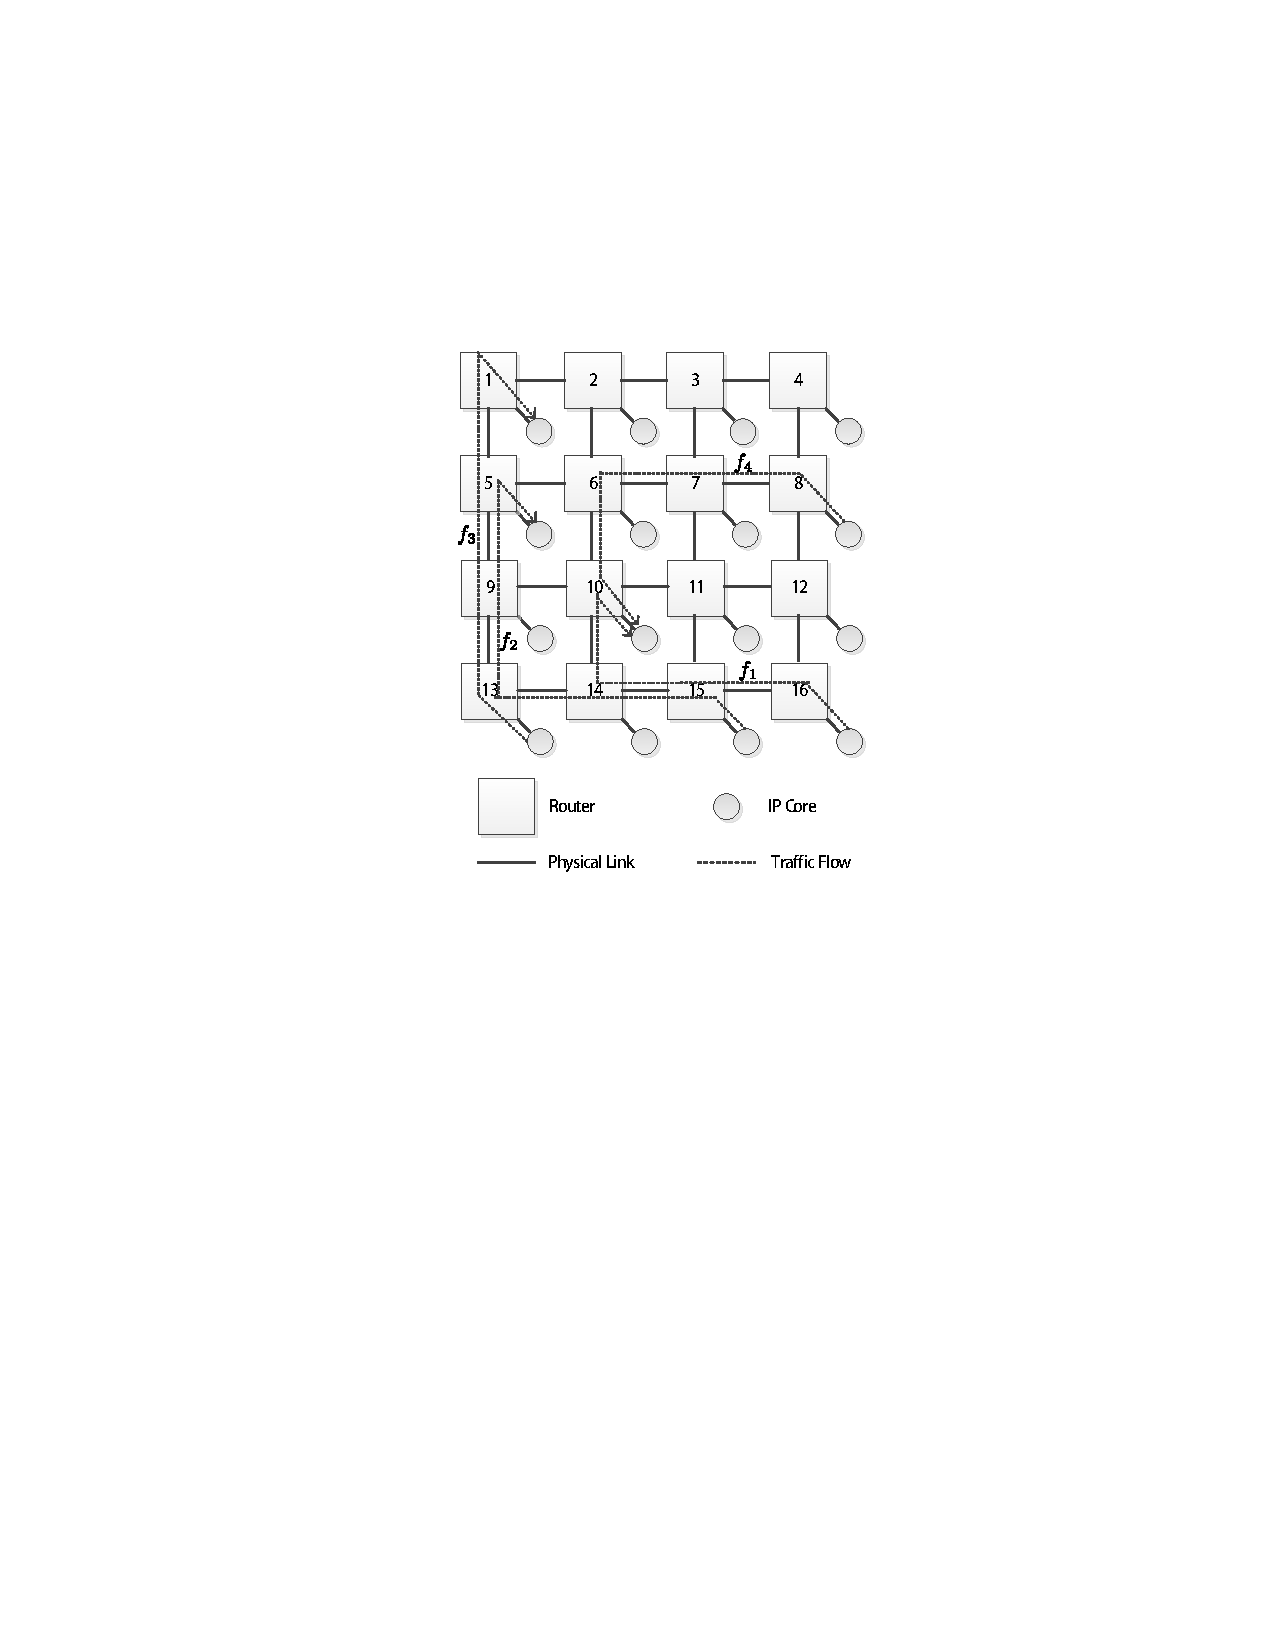
\includegraphics[scale=0.9]{figures/mesh.pdf}\\
  \caption{Mesh topology with 4 real-time traffic flows}\label{topology}
\end{figure}

\subsection{Introduction to Real-Time Calculus}
Real-time calculus is an extension of DNC \cite{1253607}, by adding the upper service curve and lower arrival curve to describe the maximal service capacity and lower arrival rate. It is the mathematical basis of Modular Performance Analysis (MPA) \cite{Wandeler2006System} technique used for real-time task scheduling. Here we only present the definition of RTC arrival curve and service curve, for more details about this theory, please refer to \cite{1253607}.
\begin{definition}[Real-Time Arrival Curve]
Let $R[s,t)$ denote the number of events that arrived in the time interval $[s,t)$. The lower bound and upper bound on $R[s,t)$ is called the lower arrival curve $\alpha^l$ and upper arrival curve $\alpha^u$ which satisfy
$$\alpha^l(t-s)\leq R[s,t)\leq \alpha^u(t-s),\forall s<t$$
where $\alpha^l(0)=\alpha^u(0)=0$. The RTC arrival curve for $R$ is denoted as $<\alpha^l,\alpha^u>$ for short.
\end{definition}

From the definition, we find that the upper arrival curve (corresponding to the arrival curve of DNC \cite{Boudec2001Network}) and lower arrival curve are used to characterize the upper and lower bound of arrived events within any interval $\Delta$.

\begin{definition}[Real-Time Service Curve]
Let $S[s,t)$ denote the total number of events that can be processed by the system in the time interval $[s,t)$. The lower bound and upper bound on $S[s,t)$ is called the lower service curve $\beta^l$ and upper service curve $\beta^u$ which satisfy
$$\beta^l(t-s)\leq S[s,t)\leq \beta^u(t-s),\forall s<t$$
where $\beta^l(0)=\beta^u(0)=0$. The RTC service curve for $S$ is denoted as $<\beta^l,\beta^u>$ for short.
\end{definition}

From the definition of RTC service curve, we find that the upper and lower service curve are corresponding to the maximal service curve and service curve in DNC theory \cite{Boudec2001Network}, respectively. Thus, the concatenation theorem (see Theorem 1.46 and Theorem 1.6.1 in \cite{Boudec2001Network}) for service curve and maximal service curve can also be applied to RTC service curve. In this paper, we will use the discrete time RTC arrival curve and service curve to characterize the system, since the minimal time unit in the wormhole-switched NoC is clock period $T$. Events in arrival curve and service curve refer to the arrival and service of flits, respectively. If we obtain the arrival curve $<\alpha^l,\alpha^u>$ of a specific traffic flow and the service curve $<\beta^l,\beta^u>$ provided to this flow, we can get the output arrival curve $<\alpha^{l^\prime},\alpha^{u^\prime}>$ of this flow and leftover service curve $<\beta^{l^\prime},\beta^{u^\prime}>$ for the other flows with the following equations:
\begin{equation}\label{alphal}
\alpha^{l^\prime}=\lfloor\min\{(\alpha^l\oslash\beta^u)\otimes\beta^l,\beta^l\}\rfloor
\end{equation}
\begin{equation}\label{alphau}
\alpha^{u^\prime}=\lceil\min\{(\alpha^u\otimes\beta^u)\oslash\beta^l,\beta^u\}\rceil
\end{equation}
\begin{equation}\label{betal}
\beta^{l^\prime}=(\beta^l-\alpha^u)\bar{\otimes}0
\end{equation}
\begin{equation}\label{betau}
\beta^{u^\prime}=\max\{(\beta^u-\alpha^l)\bar{\oslash}0,0\}
\end{equation}
where $\lceil\cdot\rceil$, $\lfloor\cdot\rfloor$ are the ceiling operator and flooring operator, and $\otimes$, $\oslash$, $\bar{\otimes}$, $\bar{\oslash}$ are corresponding to the min-plus convolution, de-convolution, and max-plus convolution and de-convolution \cite{Boudec2001Network}, respectively.

After we obtained the arrival curve $<\alpha^l_{f_i},\alpha^u_{f_i}>$ of traffic flow $f_i$ and the service curve $<\beta_{R_j,f_i}^l,\beta_{R_j,f_i}^u>$ provided by each router $R_j$ to flow $f_i$ on its path, we can obtain the end-to-end latency and backlog bound by the following equations,
\begin{equation}\label{delay}
Delay(f_i)=H(\alpha^u_{f_i},\beta^l_{R_1,f_i}\otimes\beta^l_{R_2,f_i}\otimes\cdots\otimes\beta^l_{R_N,f_i}),
\end{equation}
\begin{equation}\label{backlog}
Delay(f_i)=V(\alpha^u_{f_i},\beta^l_{R_1,f_i}\otimes\beta^l_{R_2,f_i}\otimes\cdots\otimes\beta^l_{R_N,f_i})
\end{equation}
where $H(\cdot,\cdot)$ and $V(\cdot,\cdot)$ mean the maximal vertical and horizontal deviation, respectively.

\section{Delay Analysis and Buffer Optimization}\label{modeling}
In this section, we propose a delay analysis algorithm and a buffer optimization algorithm based the RTC based analytical model. While applying the RTC theory to build the analytical model of priority-aware wormhole-switched NoC, the following four aspects should be considered: (1) Only head flit need to be processed by RC and VA stage, the subsequent flits of a packet just follow the decision of head flit. We need specific mechanism to characterize the service provided to head and non-head flits in a unified way, so that we can simplify our RTC model. (2) Due to the on-chip buffer limitation, credit-based flow control is used as a back-pressure mechanism to prevent buffer overflow. Before analysis the end-to-end performance with Eq.(\ref{delay}) and Eq.(\ref{backlog}), we should first break the cyclic-dependence caused by flow control. (3) Our model extends the existing approach \cite{73}\cite{Qian489900} by allowing priority sharing between flows. Thus, the leftover service curve provided to lower priority flows can only be derived after all the flows with higher priority have been serviced. (4) To guarantee the tightness of our theoretical bound and reduce the computation complexity, we should collapse the collapsible sub-paths as far as possible. These four issues are discussed in the follow subsections.

\subsection{Traffic Model}\label{traffic}
In a CMP or SoC system interconnected with NoC, the communication between each pair of cores was realized by transmitting packets. Each packet is further divided into flits, which is the minimum transmission unit in wormhole-switched NoC. Denote the arrival curve $<\alpha^l(\Delta),\alpha^u(\Delta)>$ of flow as the minimum and maximum amount of flits within $\Delta$ time unit. Here, we provide two ways to obtain this arrival curve: (1) We can extract the arrival curve from the communication trace generated by a real CMP or SoC system with the sliding window method \cite{1253607}. This method analyze the time series of flits by the follow way: for each window size $\Delta$, it try to find the maximal and minimal number of arrived flits in the trace, denoted by $\alpha^l(\Delta)$ and $\alpha^u(\Delta)$, respectively. We need to mention that, the obtained arrival curve obtained by this method might not be periodic, but, it does not prevent the utilization of RTC theory. (2) If we know the inter-arrival time of packets in a flow, we can also get the arrival curve directly. For example, suppose all the packets have the same length $L$ and arrived periodically with period $P$. Then, we can obtain the service curve of this flow by simply amplifying the arrival curve for periodic event stream provided in \cite{1253607} at $y$-axis with a factor $L$, as shown in Fig. \ref{ac}. The alert readers would notice that, the flit arrival curve obtained by this way is the same as the packet arrival curve $\mathcal{P}^L(\alpha)$ \cite{Boudec2001Network}. Thus, this arrival curve can also be used to compute the end-to-end packet latency, please refer to Theorem 1.7.1 in \cite{Boudec2001Network} for more details.
\begin{figure}
  \centering
  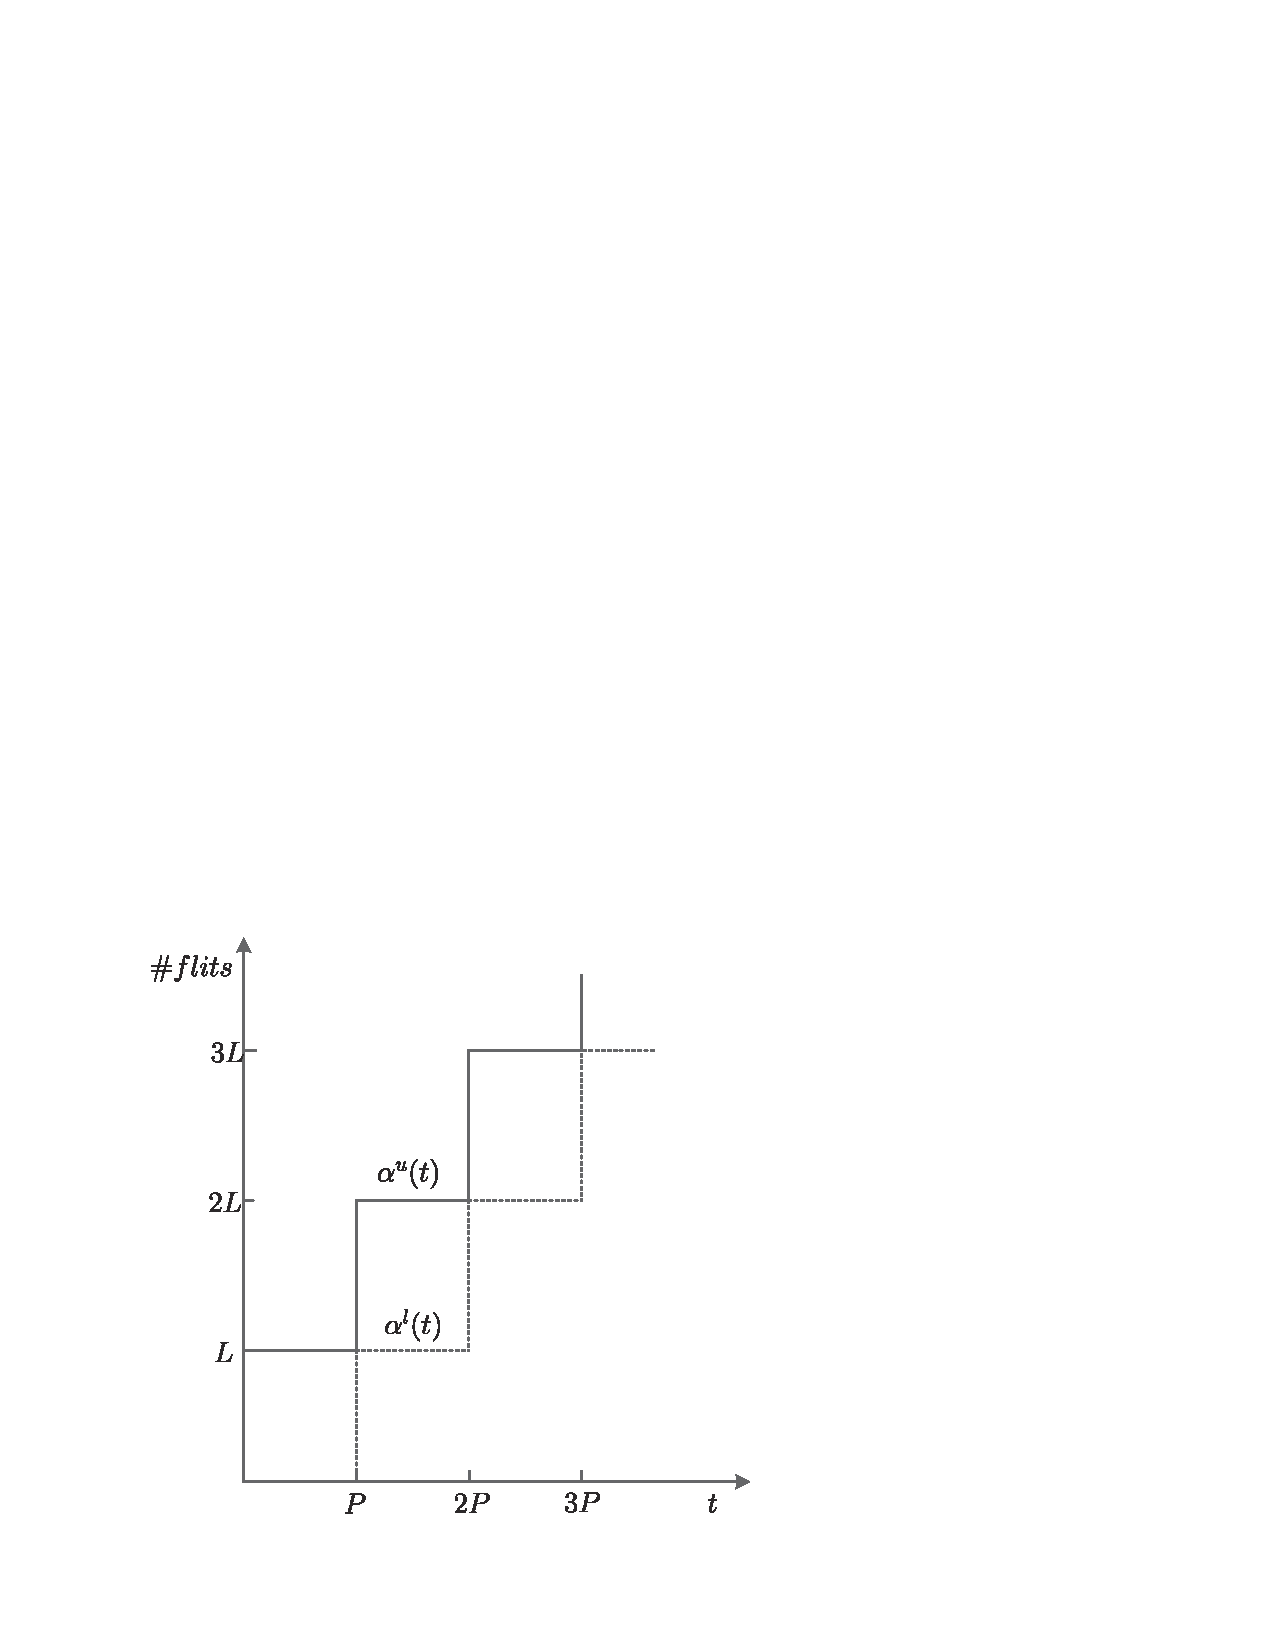
\includegraphics[scale=0.5]{figures/AC.pdf}
  \caption{Real-time calculus arrival curve for periodically arrived traffic with period $P$ and packet length $L$. The solid line and dotted line represent the upper arrival curve and lower arrival curve, respectively.}\label{ac}
\end{figure}

\subsection{Router Model}\label{router}
While modeling the routers with RTC, we can analyze the data path stage-by-stage. After found the service curve for each stages, the service curve provided by the entire router to each flow can be obtained by concatenating all the service curves of these five stages. This is significantly different with the existing DNC based model \cite{qian2009analysis,Qian489900}, where they treat the entire router as a whole and designate a Latency-Rate (LR) service curve for the router for simplicity. The advantage of our method is that, it can be easily modified to characterize the non-standard routers, by simply letting the service curve of non-existing stages to be infinity. Next, we try to obtain the service curve of all these 5 stages:
\begin{figure*}
  \centering
  \subfloat[Service curve of BW, SA and ST stages]{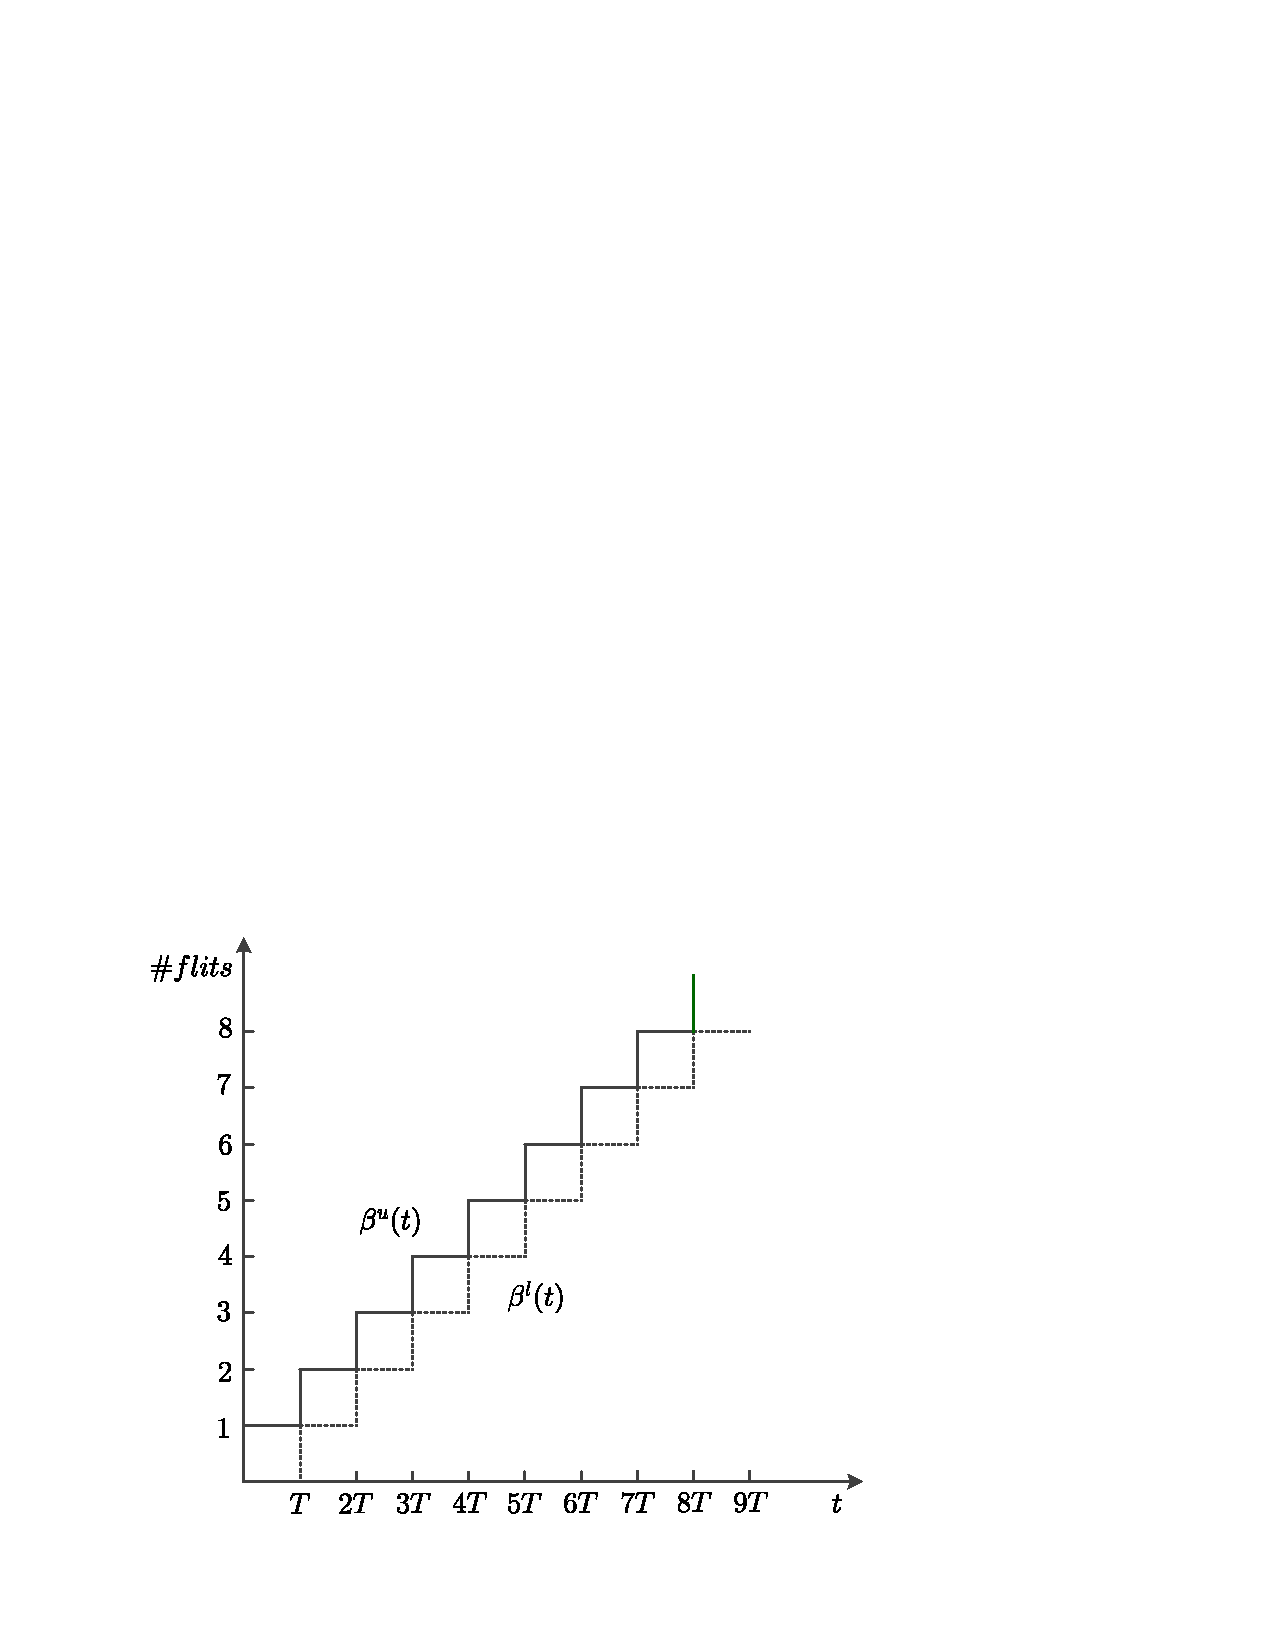
\includegraphics[scale=0.5]{figures/BW_ST_SA.pdf}\label{result1}}\hspace{10pt}
  \subfloat[Service curve of RC and VA stages]{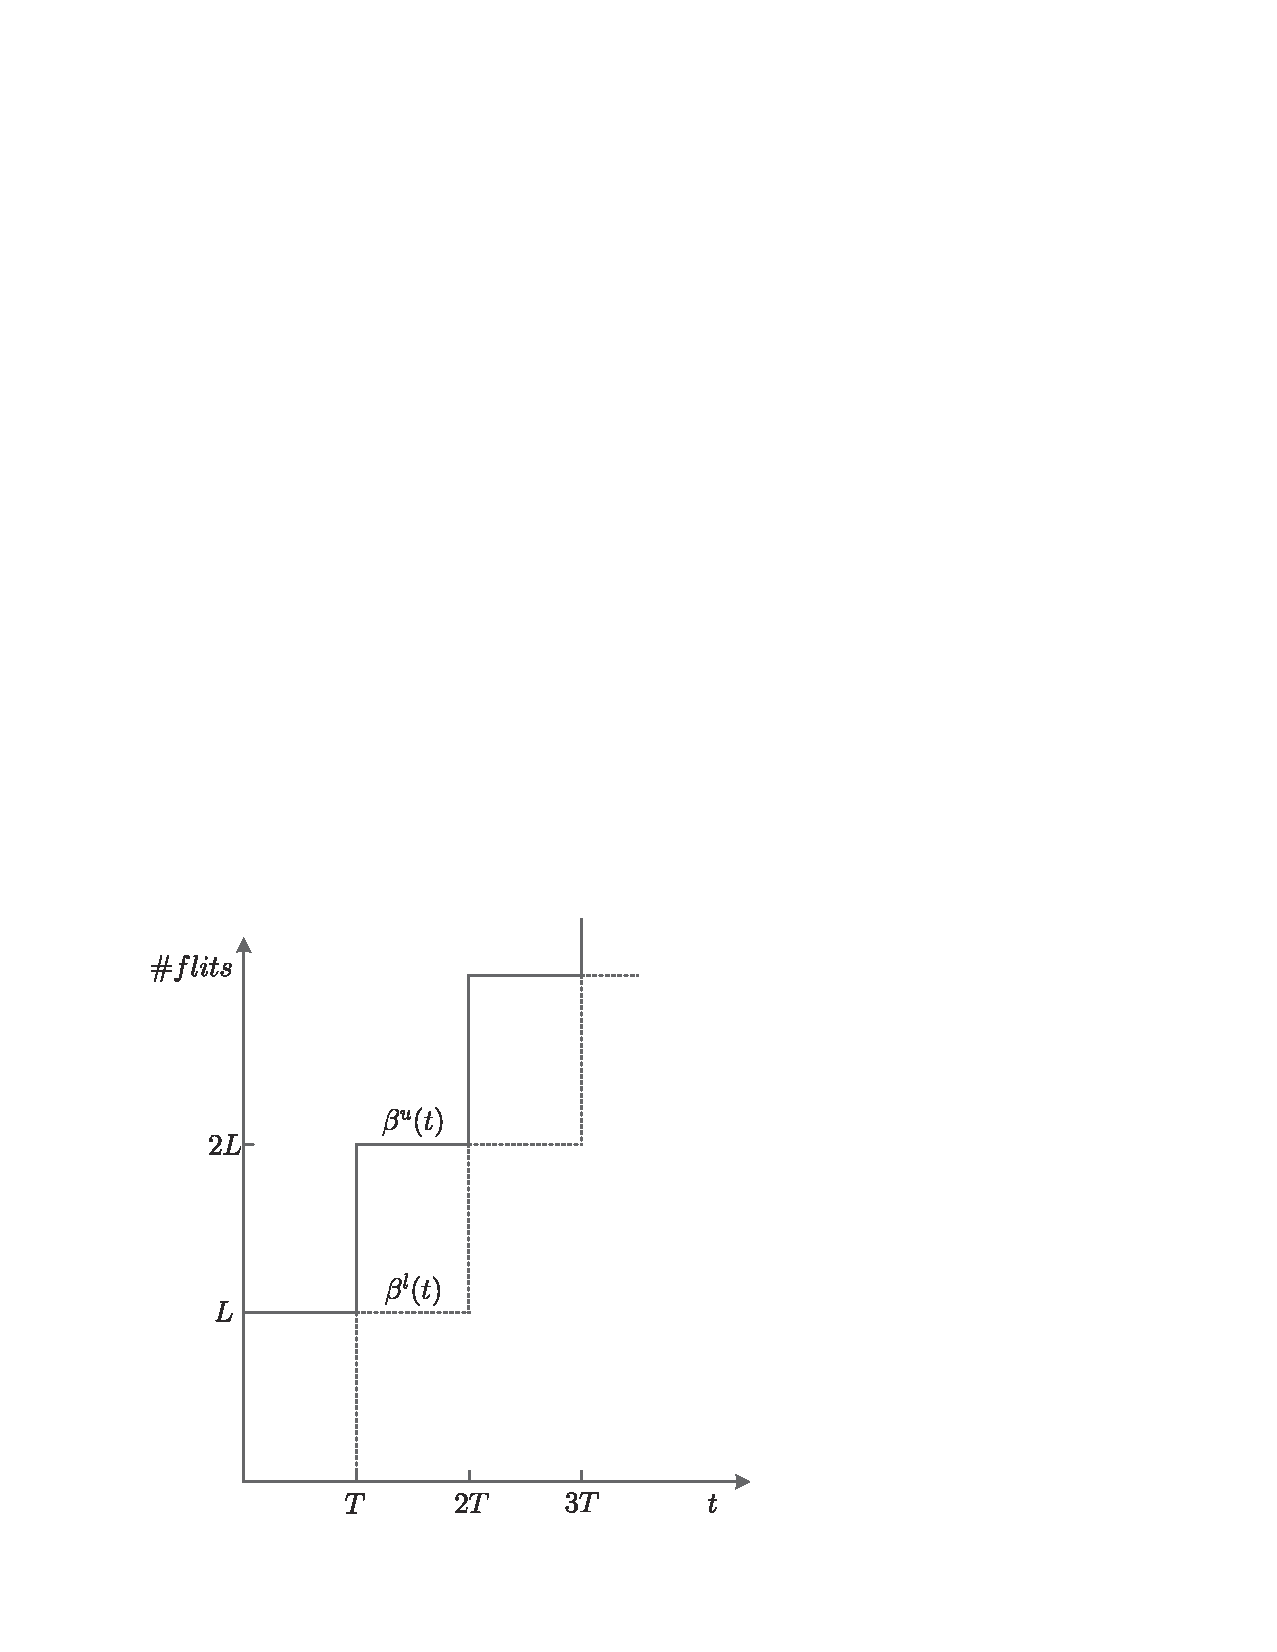
\includegraphics[scale=0.5]{figures/RC_VA.pdf}\label{result2}}
  \caption{Service model for each pipeline stages. The solid lines and dotted lines represent the upper service curves and lower service curves, respectively.}
\end{figure*}

(1) BW stage and ST stage: all the flits within a traffic flow will traverse these two stages, and experience a fixed delay $T$. Take the BW stage as an example, because this stage outputs one flit at each cycle $T$. For any time interval of length less than $T$, the maximum and minimal number of flits that can be seen are one and zero, respectively. Similarly, for any time interval of length greater than $T$, the maximum and minimal number of flits that can be seen are two and one, respectively. The resulted service curves, i.e. $<\beta^l_{BW},\beta^u_{BW}>$ and $<\beta^l_{ST},\beta^u_{ST}>$, are shown in Fig. \ref{result1}.

(2) RC stage and VA stage: only the head flit should traverse these two stages. Suppose the packet length is $L$, a sophisticated solution to construct service curve for these two stages is that, since the traverse latency for the non-head flit is $0$ cycle, we can view these two stages can provide service for all the $L$ flits within $T$ period. Then, we can get the equivalent service curve for these two stages with the same method as BW and ST stages, i.e. $<\beta^l_{RC},\beta^u_{RC}>$ and $<\beta^l_{VA},\beta^u_{VA}>$, as shown in Fig. \ref{result2}.

(3) SA stage: each output port in the wormhole-switched NoC has a SA scheduler to schedule the switch traversal at each cycle. Thus, following the same approach as BW and ST stage, we can get the service curve $<\beta_{SA}^l,\beta_{SA}^u>$ provided by SA stage to all the contention flows, as shown in Fig. \ref{roundrobin}a. For the fixed-priority based scheduling policy, switch allocators provide service for high priority flows first, and flows with the same priority will be served with Round-Robin order. The unserved flows will be imposed an additional latency $T$ due the failure of switch arbitration.

Denote by $<\beta_{SA,R_i,f_j}^l,\beta_{SA,R_i,f_j}^u>$ the service curve provided to flow $f_j$ by SA stage of router $R_i$, the equivalent service curve of router $R_i$ provided to $f_j$, i.e. $<\beta_{R_i,f_j}^l,\beta_{R_i,f_j}^u>$, can be obtained by concatenating the service curves of all the 5 stages together:
$$\beta_{R_i,f_j}^l=\beta_{BW}^l\otimes\beta_{RC}^l\otimes\beta_{VA}^l\otimes\beta_{SA,R_i,f_j}^l\otimes \beta_{ST}^l,$$
$$\beta_{R_i,f_j}^u=\beta_{BW}^u\otimes\beta_{RC}^u\otimes\beta_{VA}^u\otimes\beta_{SA,R_i,f_j}^u\otimes \beta_{ST}^u.$$

The alert readers would notice that, the contention of different flows only occurs at SA stage. Thus, if we obtained the service curve provided by SA stage to flow $f_j$, we can obtain the service curve of router directly. To obtain the service curve $<\beta_{SA,R_i,f_j}^l,\beta_{SA,R_i,f_j}^u>$, we should consider the following two cases:

(a) all the flows contending with $f_j$ at $R_i$ have lower priorities. For the synchronize router architecture, leftover service curve after serving higher priority flows is provided to $f_j$ totally. But for an asynchronous architecture, we should take the inference from low-priority flows into consideration. For example, a flit from $f_j$ arriving at SA stage just after a flit from lower priority gotten granted has to stall for a cycle. At this circumstance, the actual service curve obtained by flow $f_j$ is
\begin{equation}\label{nonpreemptbetal}
\beta^{l}_{SA,R_i,f_j}=\max\{0,\beta^{l^\prime}_{SA,R_i,f_j}-1\}
\end{equation}
where $\beta^{l^\prime}_{SA,R_i,f_j}$ is the leftover service curve calculated with Eq.(\ref{betal}). Similarly, a flow with higher priority than $f_j$ can also be blocked by $f_j$ for a cycle. Thus, denote by $\beta^{u^\prime}_{SA,R_i,f_j}$ the service curve calculated with Eq.(\ref{betau}), the actual upper service curve obtained by flow $f_j$ is
\begin{equation}\label{nonpreemptbetau}
\beta^{u}_{SA,R_i,f_j}=\min\{\beta^{u}_{SA,R_i,f_j},\beta^{u^\prime}_{SA,R_i,f_j}+1\}.
\end{equation}

(b) there exists some contention flows with the same priority as $f_j$, and the leftover service curve after serving flows with high priority than $f_j$ is $<\beta_{SA,R_i}^{l^\prime},\beta_{SA,R_i}^{u^\prime}>$. Denote by the set of contention flows at router $R_i$ with the same priority as $f_j$ as $\Theta_{R_i,f_j}$, and let $N_{R_i,f_j}$ be the number of flows in $\Theta_{R_i,f_j}$. Then, the service curve provided to $f_j$ is $<\lfloor\beta^l_{SA,R_i}/N_{R_i,f_j}\rfloor,\lceil\beta^u_{SA,R_i}/N_{R_i,f_j}\rceil>$, since all the flows in $\Theta_{R_i,f_j}$ got service in Round-Robin order. This is slightly different from the conventional continuous time model which is $<\beta^l_{SA,R_i}/N,\beta^u_{SA,R_i}/N>$, this is because our model is flit-level preemptive. An example with two flows with the same priority is shown in Fig. \ref{roundrobin}. After serving by all the flows in $\Theta_{R_i,f_j}$, the leftover service capacity for low priority flows can be obtained by applying Eq.(\ref{betal}) and Eq.(\ref{betau}).
\begin{figure*}
  \centering
  % Requires \usepackage{graphicx}
  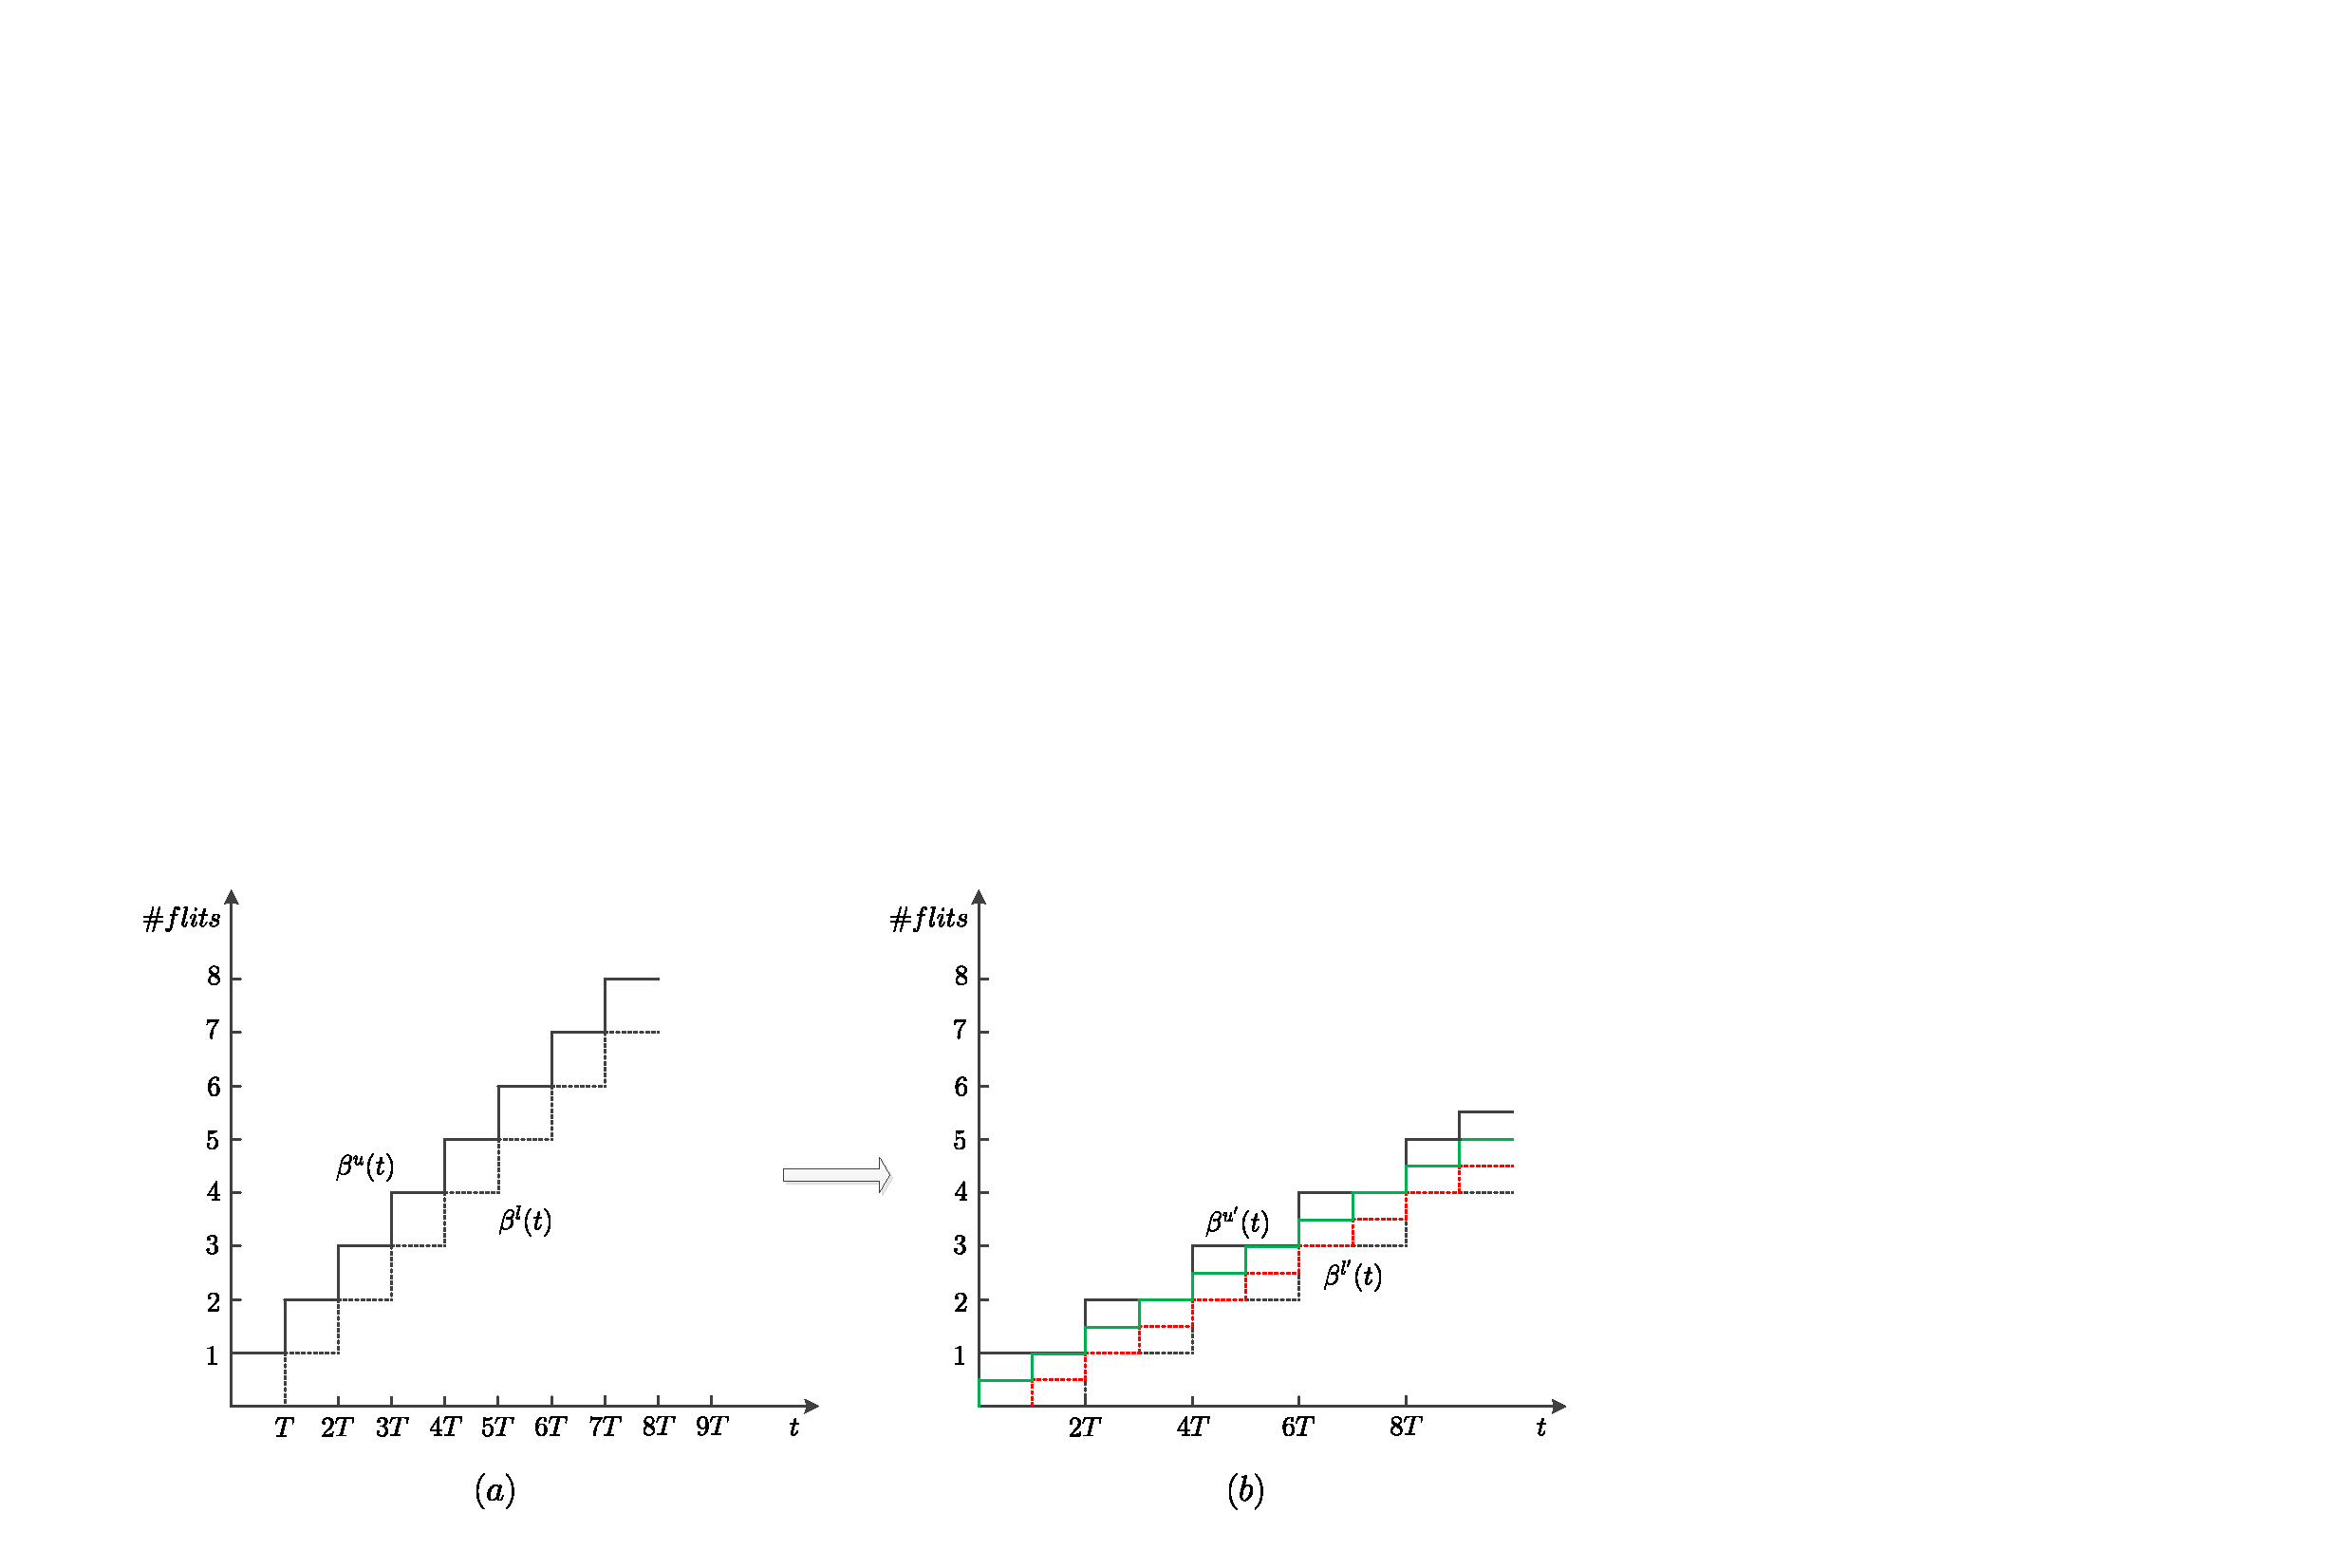
\includegraphics[scale=0.5]{figures/RoundRobin.pdf}\\
  \caption{Service curve of SA stage for two flows with the same priority under Round-Robin scheduling policy. (a) Service capacity of SA stage. (b) Upper and lower service curve provided to each contending flow, corresponding to the solid line and dotted line; the solid green line and dotted red line represent the unrounded upper and lower service curves.}\label{roundrobin}
\end{figure*}

\subsection{Upper Service Curve for Flow Controller}\label{flowcontrol}
Credit-based flow control introduces cyclic-dependence between the adjacent routers, and leads to the self-blocking within a flow due to the insufficiency of buffer space at the downstream router. Historically, the effect of self-blocking is computed numerically by fixed-point iteration \cite{schioler2005network} or symbolically analyzed by the transformation from marked dataflow graph \cite{Thiele:2009:MPA:1629335.1629353}. In this paper, we try to tackle the same problem with another solution. This is motivated by \cite{qian2009analysis}, where the authors abstract the flow control as a component providing a service curve, and the equivalent service curve (corresponding to the lower service curve of RTC) of this flow controller was obtained by applying some basic dioid algebra. In this section, we follow the same procedure in \cite{qian2009analysis} to derive the upper service curve of flow controller. The obtained upper service curve together with the lower service curve derived in \cite{qian2009analysis} enables us to break the dependence loop caused by credit-based flow control and build a comprehensive performance model with RTC. To make the question clear, we take flow $f_2$ as an example to demonstrate this method. The scheduling network of flow $f_2$ is plotted in Fig. \ref{f2}, we ignore $f_4$ and the flow control of other flows for simplicity. We assume that, the destination NI has sufficient large input buffer, thus there is no flow controller between the router and destination NI. But, to prevent the buffer overflow, there must be a flow controller between input NI and router. Denote by the output arrival process (i.e. the amount of arrived flits by time $t$) of router $R_9$, injection process (actually injected flits by time $t$) and departure process of router $R_{5}$ as $A(t)$, $I(t)$ and $D(t)$, respectively. We try to derive the service curve of flow controller at router $R_9$, as shown in the following Theorem.
\begin{figure*}
  \centering
  % Requires \usepackage{graphicx}
  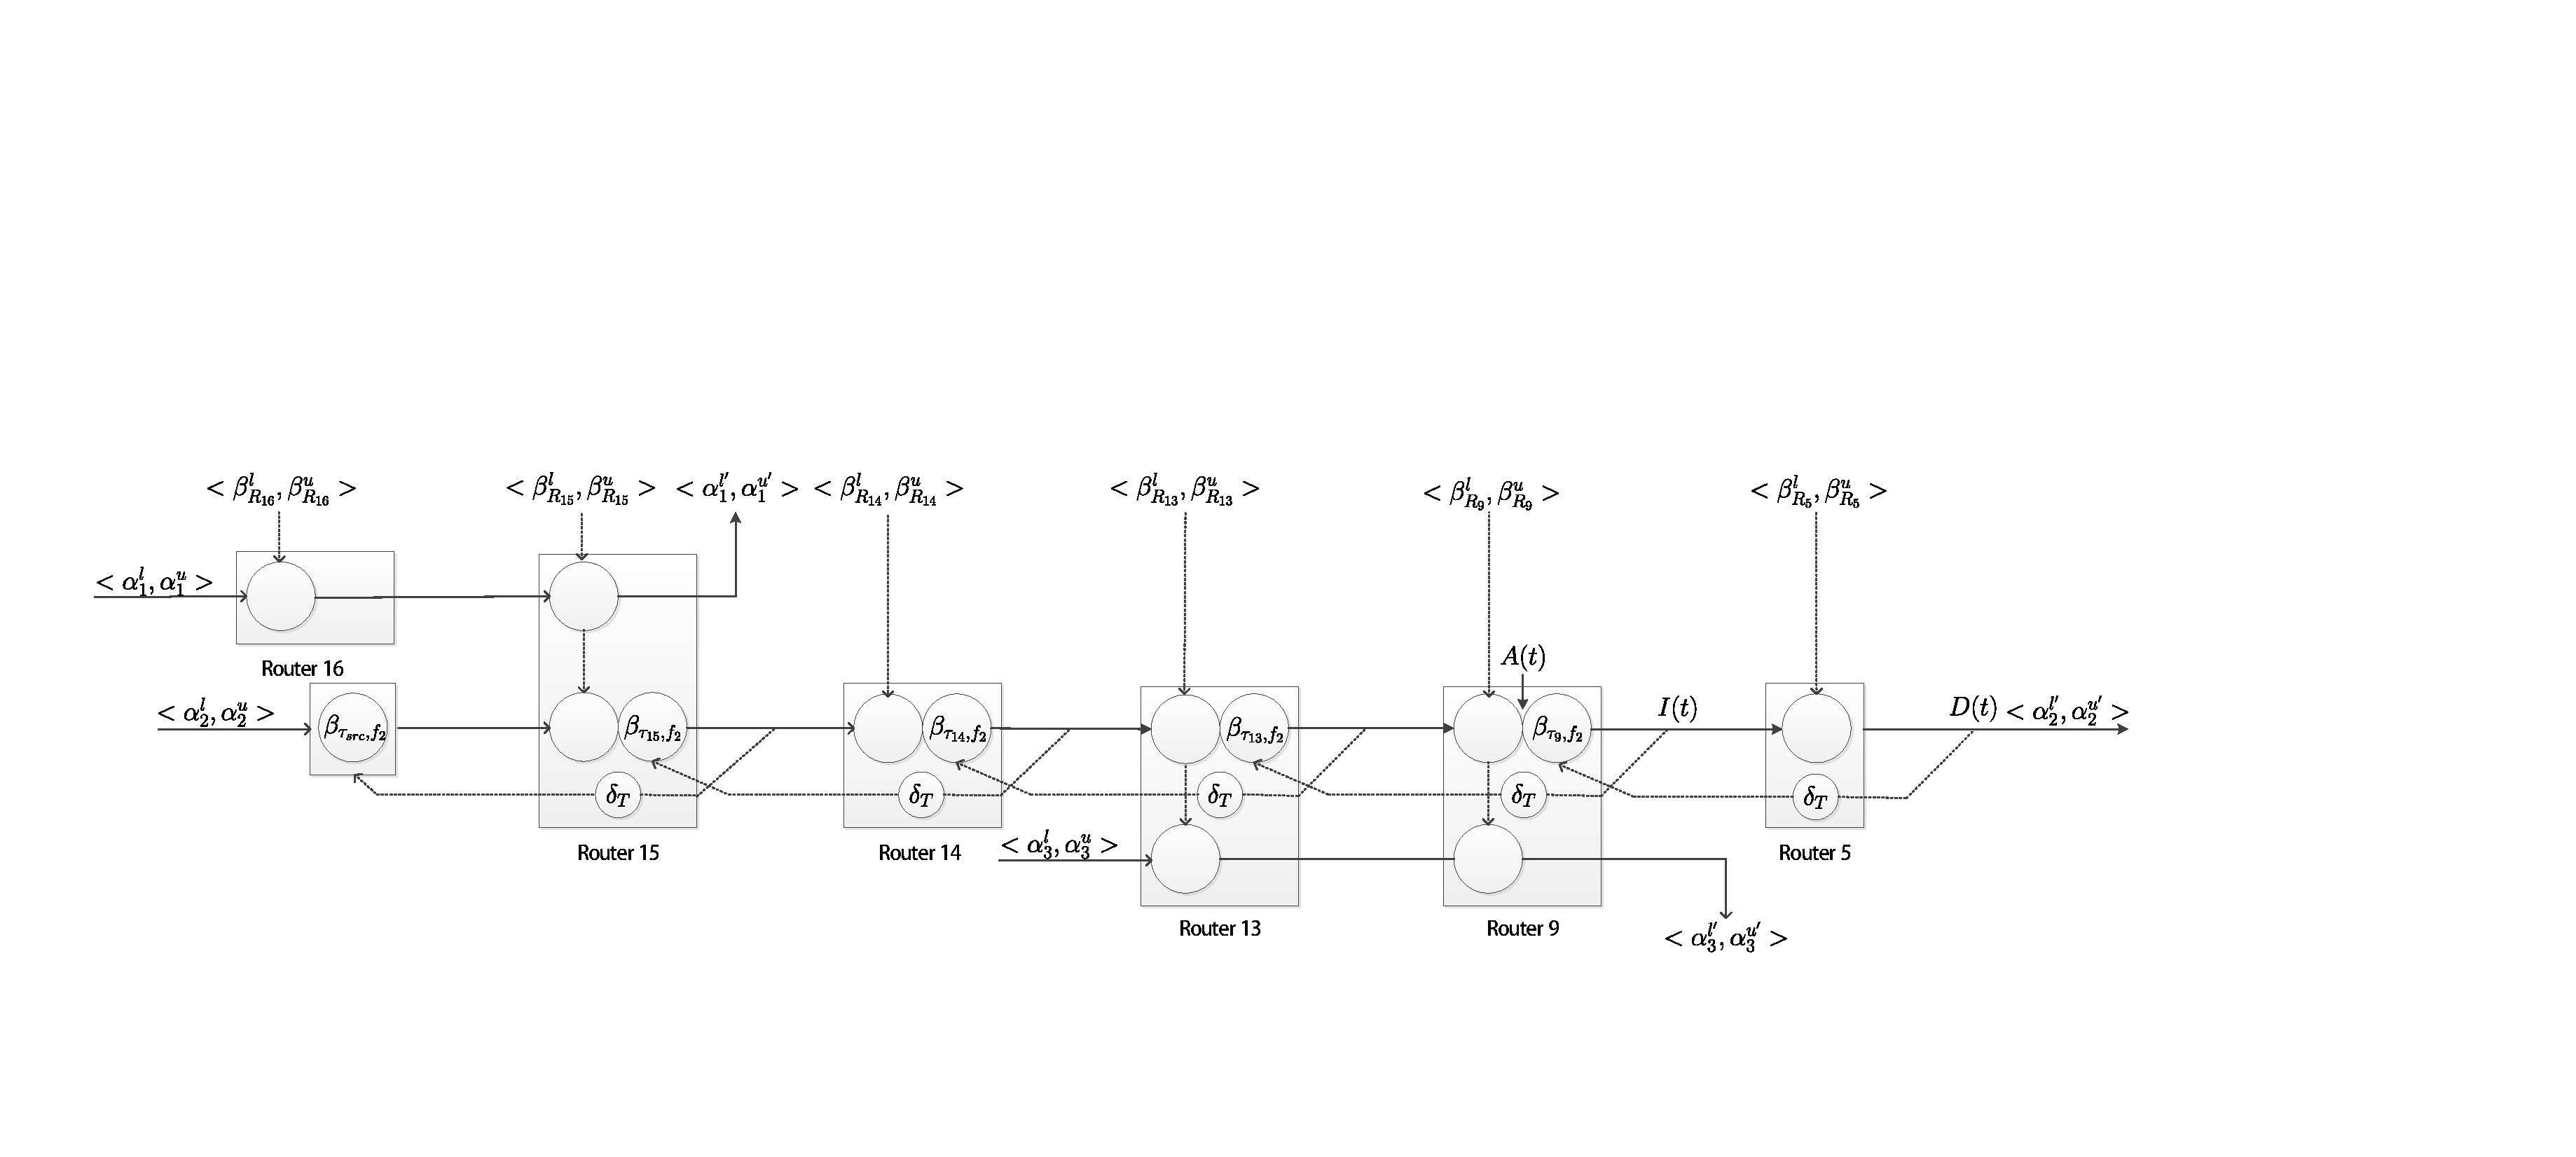
\includegraphics[scale=0.35]{figures/f2.pdf}\\
  \caption{Scheduling network model for flow $f_2$}\label{f2}
\end{figure*}

\begin{theorem}\label{credit}
Suppose each router provide an upper service curve $\beta^u$, the virtual channel depth of each router is $B$, and the feedback delay is $T$, then the flow controller provides an equivalent upper service curve $\beta^{u}_\tau$, where $$\beta^{u}_\tau(t)=\overline{\beta^u\otimes\delta_T(t)+B}$$
and $\bar{f}$ is the sub-additive closure of $f$, i.e. $\bar{f}=\inf_{n\geq 0}\{f^{(n)}\}$ and $f^{(0)}=\delta_0(t)$\footnote{$\delta_T(t)=+\infty$ for $\forall t>T$, and 0 otherwise.}.
\end{theorem}
\begin{IEEEproof}
The feedback link can be represented as a network element providing upper service curve $\delta_T(t)$. Next, we applying the same idea as \cite{qian2009analysis} to derive the upper service curve this flow controller. We know that, $I(t)=\min\{A(t),D^\prime(t)+B\}$, where $D^\prime=D\otimes\delta_T$. Denote by the service curve of router is $\beta^u$, thus $D(t)\leq I\otimes \beta^u(t)$. Bring $I(t)$ and $D^\prime(t)$ into this equation, we get
\begin{eqnarray*}
D(t)&\leq& I\otimes \beta^u(t)\\
&\leq& \min\{A\otimes \beta^u(t),D\otimes\delta_T\otimes \beta^u(t)+B\}.
\end{eqnarray*}
By applying Theorem 4.31 in \cite{Boudec2001Network}, we have
$$D\leq A\otimes \beta^u\otimes\overline{\beta^u\otimes\delta_T+B}.$$
Thus,
\begin{eqnarray*}
  I&=& \min\{A,D^\prime+B\}\\
  &\leq& \min\{A,D\otimes\delta_T+B\}\\
  &\leq& \min\{A,A\otimes \beta^u\otimes\overline{\beta^u\otimes\delta_T+B}\otimes\delta_T+B\}\\
  &=& \min\{A\otimes \delta_0,A\otimes (\beta^u\otimes\delta_T+B)\otimes\overline{\delta_T\otimes\beta^u+B}\}\\
  &=& A\otimes\overline{\beta^u\otimes\delta_T+B}.
\end{eqnarray*}
which implies that, the flow controller has an equivalent upper service curve $\overline{\beta^u\otimes\delta_T+B}$.
\end{IEEEproof}

Theorem \ref{credit} derives the upper service curve of a single flow controller, and we can get the service curve of a router chain by applying Theorem
\ref{credit} iteratively. As shown in Fig. \ref{f2}, the downstream routers' service curve can affect the service curve of flow controller at upstream. Hence, we should first derive the service curve of $f_2$ obtained at each router with the method mentioned in Subsection \ref{router}, and then compute the service curve of flow controller from destination to source. Service curve obtained at Router $R_{15}$ to flow $f_2$ can be derived by applying Eq.(\ref{betal}) and Eq.(\ref{betau}), since $f_2$ is a lower priority flow at $R_{15}$. Router $R_{13}$, $R_{9}$ and $R_{5}$ provide all their service curves to $f_2$ because $f_2$ is the highest priority flow at these routers. Denote by the service curve of flow controller obtained by Theorem \ref{credit} at router $R_{9}$ is $<\beta_{\tau_9}^l,\beta_{\tau_9}^u>$, by applying the concatenation theorem, we can obtain the equivalent service curve of router $R_{9}$ are $<\beta_{R_9}^l\otimes\beta_{\tau_9}^l,\beta_{R_9}^u\otimes\beta_{\tau_9}^u>$. Then, by applying Theorem \ref{credit}, we can get the service curve of flow controller at router $R_{13}$, $R_{14}$, $R_{15}$ and NI that connected to $R_{15}$ iteratively.

\subsection{Collapsible Sub-Path}
We have build the traffic model, router model and flow control model in the previous subsection. Before we give the performance evaluation algorithm, we first consider the follow scenario. Take $f_2$ and $f_3$ in Fig. \ref{topology} as an example, they content the output link at both router $R_{13}$ and $R_{9}$. Denote by $B_{R_9,f_2}$ the buffer depth of $R_{9}$ allocated to flow $f_2$, $<\beta_{R_{13},f_2}^l,\beta_{R_{13},f_2}^u>$ and $<\beta_{R_{9},f_2}^l,\beta_{R_{9},f_2}^u>$ the service curve of $R_{13}$ and $R_{9}$ provided to flow $f_2$, $<\beta_{\tau_{13},f_2}^l,\beta_{\tau_{13},f_2}^u>$ the service curve for flow controller of router $R_{13}$, $<\alpha_{R_{13},f_2}^l,\alpha_{R_{13},f_2}^u>$ and $<\alpha_{R_{13},f_3}^l,\alpha_{R_{13},f_3}^u>$ the arrival curve of $f_2$ and $f_3$ at router $R_{13}$. The question is: when $B_{R_9,f_2}$ is sufficiently large so that $\beta_{R_{13},f_2}^l\otimes\beta_{\tau_{13},f_2}^l=\beta_{R_{13},f_2}^l$ and $\beta_{R_{13},f_2}^u\otimes\beta_{\tau_{13},f_2}^u=\beta_{R_{13},f_2}^u$, how to derive the leftover service curve for $f_3$ at $R_{13}$ and $R_9$, and obtain a tight delay and backlog bound of $f_3$ efficiently?

An intuitive solution is that calculating the leftover service curve router by router: Firstly, obtaining the leftover service curve of $R_{13}$ by applying Eq.(\ref{betal}) and Eq.(\ref{betau}); Secondly, deriving the output arrival curve $<\alpha_{R_{9},f_2}^{l^\prime},\alpha_{R_{9},f_2}^{u^\prime}>$ of $f_2$ by applying Eq.(\ref{alphal}) and Eq.(\ref{alphau}); Thirdly, the leftover service curve of $R_9$ can be easily obtained by applying Eq.(\ref{betal}) and Eq.(\ref{betau}); And finally, the leftover service curve for $f_3$ at $R_{13}$ and $R_9$ can be easily obtained by concatenation theorem of service curve. Another solution is: we can substitute $R_{13}$ and $R_{9}$ by a virtual router $R_{13,9}$ providing service curve $<\beta_{R_{13},f_2}^l\otimes\beta_{R_{13},f_2}^l,\beta_{R_{13},f_2}^u\otimes\beta_{R_{13},f_2}^u>$, since $B_{R_9,f_2}$ is sufficiently large and the flow control between $R_{13}$ and $R_9$ can be ignored, as shown in Fig. \ref{collapse}. Then, the leftover service curve $f_3$ obtained at $R_{13}$ and $R_{9}$ can be directly obtained by applying Eq.(\ref{betal}) and Eq.(\ref{betau}). Compared with previous method, it eliminates the calculation of intermediate arrival curve, and compute the equivalent service curve by just invoke Eq.(\ref{betal}) and Eq.(\ref{betau}) once, which is calculation efficient. We will also demonstrate in Section \ref{experiments} that, this method can achieve tighter performance bound compared with the former method.
\begin{figure}
  \centering
  % Requires \usepackage{graphicx}
  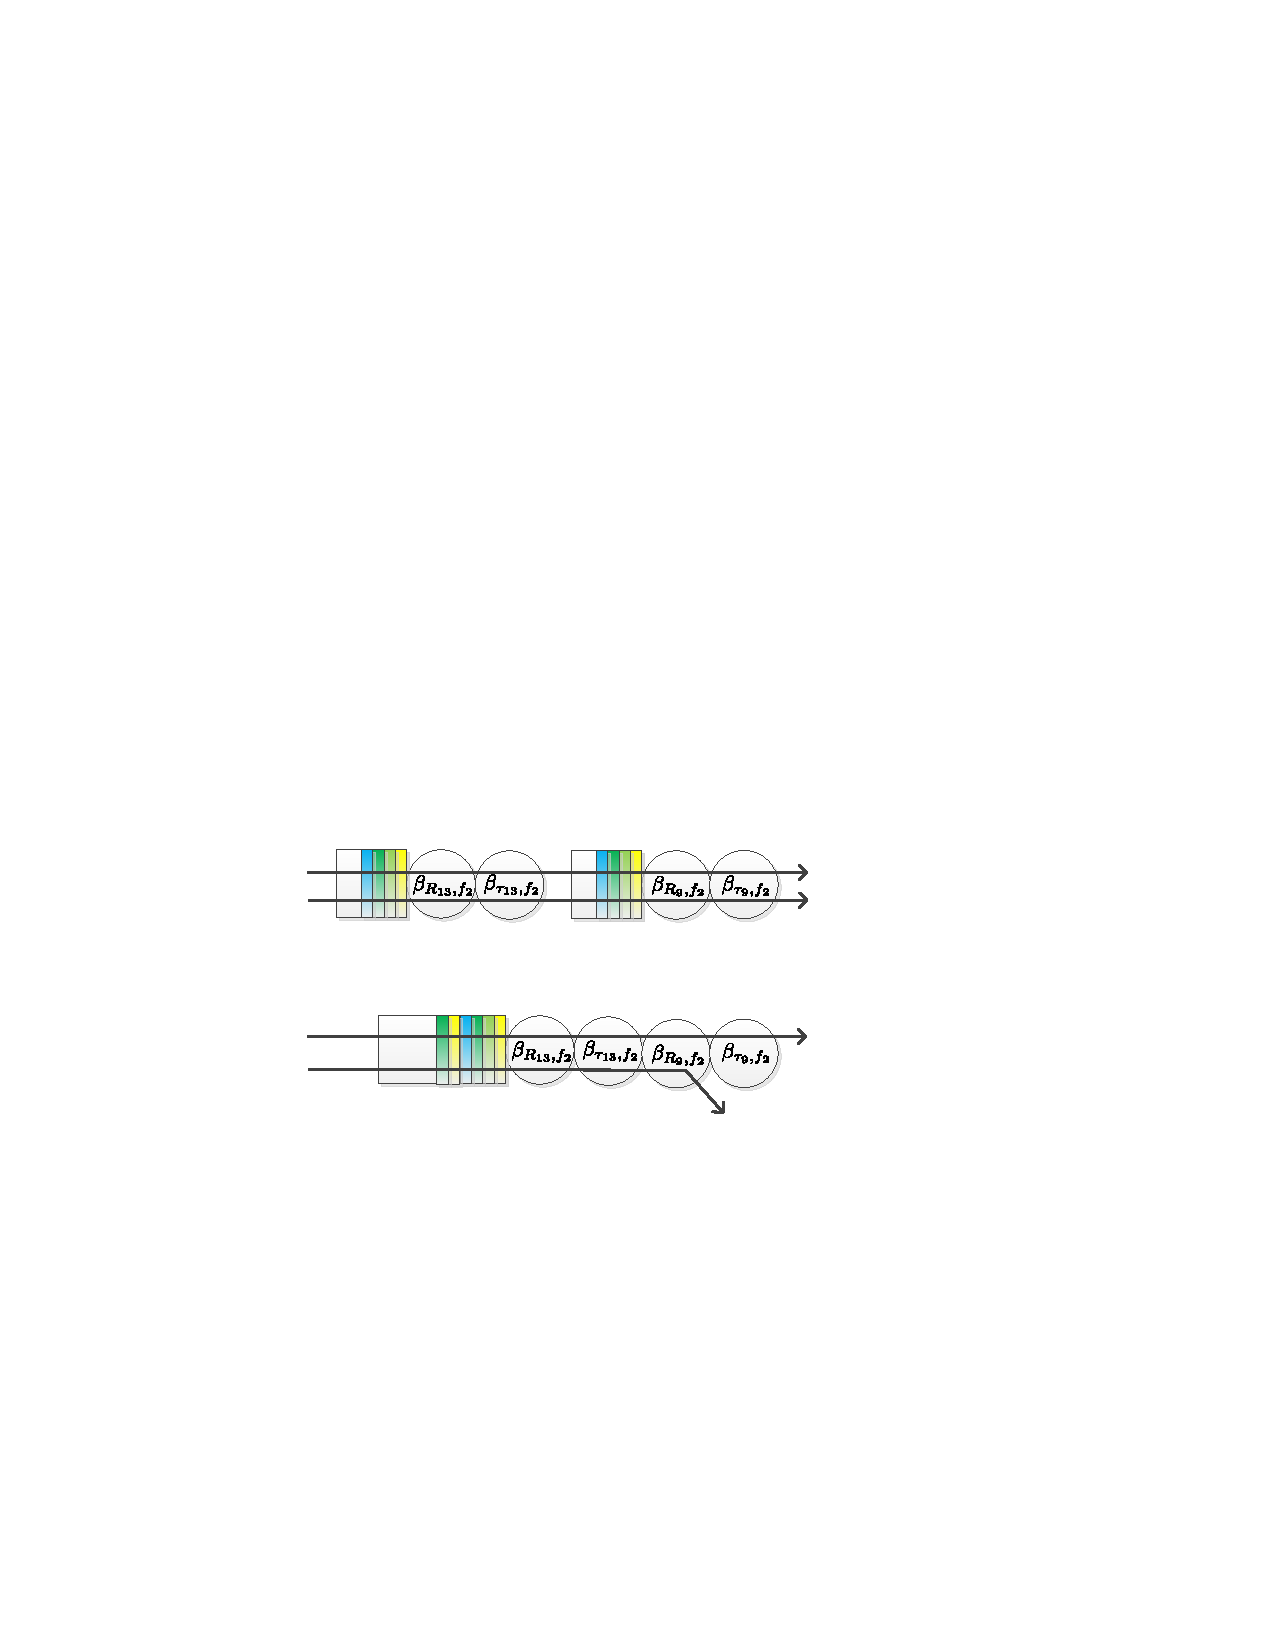
\includegraphics[scale=0.5]{figures/collapse.pdf}\\
  \caption{Collapsible sub-path of $f_2$. Since the flow control between $R_{13}$ and $R_9$ can be ignored, they are replaced by a single virtual router $R_{13,9}$.}\label{collapse}
\end{figure}

Next, we formalize this observation and propose the concept of collapsible Sub-Path (CSP). After identifying all the CSPs on the path of a flow, the optimized performance calculation method can be applied.
\begin{definition}[Collapsible Sub-Path]
The collapsible sub-path of flow $f$, denoted by $CSP(f)$, is a sub-path of $f$ satisfying the follow conditions:
\begin{enumerate}
  \item all the routers $R_i$ on this sub-path, except the last one, satisfy $\beta_{R_{i},f}^l\otimes\beta_{\tau_{i},f}^l=\beta_{R_{i},f}^l$ and $\beta_{R_{i},f}^u\otimes\beta_{\tau_{i},f}^u=\beta_{R_{i},f}^u$.
  \item $CSP(f)$ is also a sub-path of all the flows in $\Omega_{f}$, where $\Omega_{f}$ is the set of contention flows with lower priorities on this sub-path.
\end{enumerate}
\end{definition}

For the high priority flows, the process of calculating the end-to-end equivalent service curve is also a collapsing process. But, to compute the leftover service curve at some routers, we have to know the arrival curve at these routers. As implied previously, instead of the router-by-router calculation, we can leverage the concept of CSP and replace all the routers on $CSP(f)$ with a single virtual router providing service curve $<\otimes_{R_i\in CSP(f)}\beta_{R_i,f}^l,\otimes_{R_i\in CSP(f)}\beta_{R_i,f}^u>$. For a CSP with $N$ routers, this method reduces $N-1$ times calculation of arrival curve and leftover service curve, the leftover service curve calculation is greatly simplified, and the accuracy of performance bound is also improved due to the well-known ``Pay-Burst-Only-Once" phenomenon in DNC theory \cite{Boudec2001Network}.

\subsection{End-to-End Latency}
After obtained the traffic model, router model and flow control model, compute the end-to-end latency is still a non-trivial task. The follow four aspects should be considered carefully: (1) We should always compute the end-to-end latency by collapsing all the CSP to a single virtual node, as the hop-by-hop computation will lead to a looser bound; (2) In the fixed-priority flit-level preemptive NoC, only the leftover service curve can be used by the low priority flows, thus, our computation must start from higher priority flows to lower priority; (3) Before computing the leftover service curve for lower priority flows, we must ensure that all the higher priority flows has been served; (4) The computed service curve for flow controller can only be applicable for specific flow, and we should compute these curves for each flows.

Keeping these four aspects in mind, we propose the performance evaluation algorithm, as shown in Algorithm \ref{alg:equivalentservicecurve}. Here are some explanation about our algorithm: suppose the entire NoC is represented as a directional topology graph $G:\ V\times E$, where $V$ and $E$ represent the set of routers and links, respectively. For each link $e_{i,j}\in E$ represent there is a physical channel between router $R_i$ and router $R_j$, $e_{i,j}\neq e_{j,i}$ since the topology graph is a directional graph. The set of all the flows in the network is denoted as $\mathcal{F}$, and each flow $f_i\in\mathcal{F}$ has a fixed-priority $P_i$. To simplify the description of our algorithm, we assume that $P_i\geq P_j$ holds for $\forall$ $i\geq j$. The set of routers a flow $f_i$ traversed is denoted as $\mathcal{R}_i$, and the set of links a flow $f_i$ traversed is denoted as $\Gamma_i$. If there exists interference between flow $f_i$ and $f_j$, then $\Gamma_i\wedge\Gamma_j\neq\Phi$ and the set of contention routers is $\mathcal{R}_i\wedge\mathcal{R}_j$. The arrival curve of $f_i$ at router $R_j$ is $<\alpha_{R_j,f_i}^l,\alpha_{R_j,f_i}^u>$, and the leftover service curve of SA stage at router $R_j$ is denoted as $<\beta_{SA,R_j}^{l^\prime},\beta_{SA,R_j}^{u^\prime}>$ (initially, $\beta_{SA,R_j}^{l^\prime}=\beta_{SA,R_j}^{l}$ and $\beta_{SA,R_j}^{u^\prime}=\beta_{SA,R_j}^{u}$). For all the router $R_j$ along the path of flow $f_i$, denote by the contention flows with the same priority as $f_i$ as $\Theta_{R_j,f_i}$, the set with lower priority flow as $\Omega_{R_j,f_i}$, and the buffer size as $B_{R_j,f_i}$. In addition, let $N_{R_j,f_i}$ and $N_{f_i}$ be the number of flows in $\Theta_{R_j,f_i}$ and the number of routers that $f_i$ traversed.
\begin{algorithm}
\caption{End-to-End Latency Analysis Algorithm}
\label{alg:equivalentservicecurve}
\begin{algorithmic}[1]
    \FOR {each flow $f_i\in\mathcal{F}$}
        \FOR {each router $R_j\in\mathcal{R}_{i}$}
            \STATE $\beta_{SA,R_j,f_i}^l=\delta_0(t)$; $\beta_{SA,R_j,f_i}^u=\delta_0(t)$;
        \ENDFOR
    \ENDFOR
    \FOR {each flow $f_i\in \mathcal{F}$ with priority order}
        \FOR {each router $R_j\in \mathcal{R}_{i}$}
            \IF {$\Theta_{R_j,f_i}\neq \emptyset$}
                \FOR {each flow $f_k\in \Theta_{R_j,f_i}$}
                    \STATE $\beta_{SA,R_j,f_k}^{l^\prime}=\lfloor\beta_{SA,R_j}^l/N_{R_j,f_i}\rfloor$;
                    \STATE $\beta_{SA,R_j,f_k}^{u^\prime}=\lceil\beta_{SA,R_j}^u/N_{R_j,f_i}\rceil$;
                \ENDFOR
            \ENDIF
            \IF {$\beta_{SA,R_j,f_i}^l=\delta_0(t)$ and $\beta_{SA,R_j,f_i}^u=\delta_0(t)$}
                \STATE $\beta_{SA,R_j,f_i}^l=\beta_{SA,R_j}^{l^\prime}$; $\beta_{SA,R_j,f_i}^u=\beta_{SA,R_j}^{u^\prime}$;
            \ENDIF
            \STATE $\beta_{R_j,f_i}^l=\beta_{BW}^l\otimes\beta_{RC}^l\otimes\beta_{VA}^l\otimes\beta_{SA,R_j,f_i}^l\otimes \beta_{ST}^l$;
            \STATE $\beta_{R_j,f_i}^u=\beta_{BW}^u\otimes\beta_{RC}^u\otimes\beta_{VA}^u\otimes\beta_{SA,R_j,f_i}^u\otimes \beta_{ST}^u$;
        \ENDFOR
        \STATE $\beta_{\tau}^l=\delta_0(t)$; $\beta_{\tau}^u=\delta_0(t)$;
        \FOR {each router $R_j\in\mathcal{R}_i$ from destination to source}
            \STATE $\beta^{l}_{\tau_j,f_i}(t)=\beta_{\tau}^l$; $\beta_{\tau}^l=\overline{\beta^l_{R_j,f_i}\otimes\beta^{l}_{\tau}\otimes\delta_T(t)+B_{R_j,f_i}}$;
            \STATE $\beta^{u}_{\tau_j,f_i}(t)=\beta_{\tau}^u$; $\beta_{\tau}^u=\overline{\beta^u_{R_j,f_i}\otimes\beta^{u}_{\tau}\otimes\delta_T(t)+B_{R_j,f_i}}$;
        \ENDFOR
        \STATE Collapse $CSP(f_i)$ and update $\Theta_{R_j,\cdot}$, $\Omega_{R_j,\cdot}$ and $\mathcal{R}_{\cdot}$;
        \STATE $Delay(f_i)=H(\alpha^u_{f_i},\beta^l_{R_1,f_i}\otimes\beta^l_{R_2,f_i}\otimes\cdots\otimes\beta^l_{R_{N_{f_i}},f_i})$;
        \STATE $\beta_{f_i}^l=\delta_0(t)$; $\beta_{f_i}^u=\delta_0(t)$;
        \FOR {For all the router $R_j$ in $\mathcal{R}_{f_i}$}
            \STATE $\beta^l=\beta^l_{f_i}\otimes\beta_{BW}^l\otimes\beta_{RC}^l\otimes\beta_{VA}^l$;
            \STATE $\beta^u=\beta^u_{f_i}\otimes\beta_{BW}^u\otimes\beta_{RC}^u\otimes\beta_{VA}^u$;
            \STATE $\alpha^l_{R_j,f_i}=\lfloor\min\{(\alpha^l\oslash\beta^u)\otimes\beta^l,\beta^l\}\rfloor$;
            \STATE $\alpha^u_{R_j,f_i}=\lceil\min\{(\alpha^u\otimes\beta^u)\oslash\beta^l,\beta^u\}\rceil$;
            \STATE $\beta_{f_i}^l=\beta_{f_i}^l\otimes\beta_{R_j,f_i}^l$; $\beta_{f_i}^u=\beta_{f_i}^u\otimes\beta_{R_j,f_i}^u$;
            \IF {$\Omega_{R_j,f_i}\neq \emptyset$}
                \IF {delay of $\forall f_k\in\Theta_{R_j,f_i}$ has been calculated}
                    \STATE $\alpha^l_{R_j,f_i}=\alpha^l_{R_j,f_i}+\sum_{f_k\in\Theta_{R_j,f_i}}\alpha^l_{R_j,f_k}$;
                    \STATE $\alpha^u_{R_j,f_i}=\alpha^u_{R_j,f_i}+\sum_{f_k\in\Theta_{R_j,f_i}}\alpha^u_{R_j,f_k}$;
                \ENDIF
                \STATE $\beta^{l^\prime}_{SA,R_j}=(\beta^l_{SA,R_j}-\alpha^u_{R_j,f_i})\bar{\otimes}0$;
                \STATE $\beta^{u^\prime}_{SA,R_j}=\max\{(\beta^u_{R_j}-\alpha^l_{R_j,f_i})\bar{\oslash}0,0\}$;
            \ENDIF
        \ENDFOR
    \ENDFOR
\end{algorithmic}
\end{algorithm}

In Algorithm \ref{alg:equivalentservicecurve}, the leftover service curve for lower priority flows should compute after all the service curve of higher priority flows have been calculated, we add the label ``Calculated" to distinguish this scenario. The overall algorithm has two embedded loops, and the computation complexity for this algorithm is $O(np)$, where $n$ and $p$ is the number of flows and the hop count of each flow. This algorithm is of pseudo-polynomial complexity due to the computation complexity of algorithmic min-plus convolution and sub-additive closure \cite{Bouillard2008}. This algorithm can be easily integrated into the RTC toolbox\cite{rtc} to compute the end-to-end latency automatically.

\subsection{Buffer Optimization}
The priority-aware NoC requires the same amount of VC as the priorities, to reduce the design cost, we need to reduce either the number of VCs with priority sharing techniques \cite{5161497} or the buffer depth of each VC. In \cite{189}, two backlog bound are derived with FLBA and LLBA, but these bounds are obtained with the assumption that, the buffer size is sufficient large so that the blocking caused by flow control can be ignored. In this section, we propose a buffer optimization algorithm taking the flow control into consideration to further improve the existing backlog bounds. We assume the application has been mapped onto the NoC, and each flow $f_i$ has been assigned to their corresponding priority $P_i$ and deadline $D_i$. Our aim is the reduce the buffer size under the constraint of deadline not be violated. Our algorithm can be used to optimize the buffer size of priority aware NoC in conjunction with the priority sharing techniques.
\begin{algorithm}
\caption{Buffer Optimization Algorithm}
\label{alg:bufopt}
\begin{algorithmic}[1]
    \FOR {All flows $f_i\in \mathcal{F}$}
        \FOR {each router $R_j\in \mathcal{R}_{i}$}
            \IF {$\Theta_{R_j,f_i}\neq \emptyset$}
                \STATE $\beta_{R_j,f_i}^l=\beta_{BW}^l\otimes\beta_{RC}^l\otimes\beta_{VA}^l\otimes\lfloor\frac{\beta_{SA,R_j}^{l^\prime}}{N_{R_j,f_i}}\rfloor\otimes\beta_{ST}^l$;
                \STATE $\beta_{R_j,f_i}^u=\beta_{BW}^u\otimes\beta_{RC}^u\otimes\beta_{VA}^u\otimes\lceil\frac{\beta_{SA,R_j}^{u^\prime}}{N_{R_j,f_i}}\rceil\otimes\beta_{ST}^u$;
            \ELSE
                \STATE $\beta_{R_j,f_i}^l=\beta_{BW}^l\otimes\beta_{RC}^l\otimes\beta_{VA}^l\otimes\beta_{SA,R_j}^{l^\prime}\otimes\beta_{ST}^l$;
                \STATE $\beta_{R_j,f_i}^u=\beta_{BW}^u\otimes\beta_{RC}^u\otimes\beta_{VA}^u\otimes\beta_{SA,R_j}^{u^\prime}\otimes\beta_{ST}^u$;
            \ENDIF
            \STATE $B^l=\inf\{B|\beta_{R_j,f_i}^l\otimes\overline{\beta_{R_j,f_i}^l\otimes\delta_T(t)+B}\geq\beta_{R_j,f_i}^l\}$;
            \STATE $B^u=\inf\{B|\beta_{R_j,f_i}^u\otimes\overline{\beta_{R_j,f_i}^u\otimes\delta_T(t)+B}\geq\beta_{R_j,f_i}^u\}$;
            \STATE $B_{R_j,f_i}=\max\{B^l,B^u\}$;
        \ENDFOR
        \STATE $curnode=Pre(end_i)$;
        \WHILE {$Pre(curnode)\neq null$}
            \STATE $\beta_{f_i}^l=\underset{R_{j}\in\mathcal{R}_i}{\otimes}(\beta^l_{R_j,f_i}\otimes\overline{\beta^l_{R_j,f_i}\otimes\delta_T+B_{R_j,f_i}})$;
            \WHILE {$H(\alpha_{f_i}^u,\beta_{f_i}^l)<D_i$}
                \STATE $B_{curnode,f_i}=B_{curnode,f_i}-1$;
                \STATE $\beta_{f_i}^l=\underset{R_{j}\in\mathcal{R}_i}{\otimes}(\beta^l_{R_j,f_i}\otimes\overline{\beta^l_{R_j,f_i}\otimes\delta_T+B_{R_j,f_i}})$;
            \ENDWHILE
            \STATE $curnode=Pre(curnode)$;
        \ENDWHILE
        \STATE $\beta_{f_i}^l=\delta_0(t)$; $\beta_{f_i}^u=\delta_0(t)$;
        \FOR {For all the router $R_j$ in $\mathcal{R}_{f_i}$}
            \STATE $\beta^l=\beta^l_{f_i}\otimes\beta_{BW}^l\otimes\beta_{RC}^l\otimes\beta_{VA}^l$;
            \STATE $\beta^u=\beta^u_{f_i}\otimes\beta_{BW}^u\otimes\beta_{RC}^u\otimes\beta_{VA}^u$;
            \STATE $\alpha^l_{R_j,f_i}=\lfloor\min\{(\alpha^l\oslash\beta^u)\otimes\beta^l,\beta^l\}\rfloor$;
            \STATE $\alpha^u_{R_j,f_i}=\lceil\min\{(\alpha^u\otimes\beta^u)\oslash\beta^l,\beta^u\}\rceil$;
            \STATE $\beta_{f_i}^l=\beta_{f_i}^l\otimes\beta_{R_j,f_i}^l$; $\beta_{f_i}^u=\beta_{f_i}^u\otimes\beta_{R_j,f_i}^u$;
            \IF {$\Omega_{R_j,f_i}\neq \emptyset$}
                \IF {delay of $\forall f_k\in\Theta_{R_j,f_i}$ has been calculated}
                    \STATE $\alpha^l_{R_j,f_i}=\alpha^l_{R_j,f_i}+\sum_{f_k\in\Theta_{R_j,f_i}}\alpha^l_{R_j,f_k}$;
                    \STATE $\alpha^u_{R_j,f_i}=\alpha^u_{R_j,f_i}+\sum_{f_k\in\Theta_{R_j,f_i}}\alpha^u_{R_j,f_k}$;
                \ENDIF
                \STATE $\beta^{l^\prime}_{SA,R_j}=(\beta^l_{SA,R_j}-\alpha^u_{R_j,f_i})\bar{\otimes}0$;
                \STATE $\beta^{u^\prime}_{SA,R_j}=\max\{(\beta^u_{R_j}-\alpha^l_{R_j,f_i})\bar{\oslash}0,0\}$;
            \ENDIF
        \ENDFOR
    \ENDFOR
\end{algorithmic}
\end{algorithm}

The path of flow $f_i$ is started from source NI (denoted by $start_i$) following a sequence of routers, and ended at destination NI (denoted by $end_i$). For any router $curnode$ on the path, denote by $Pre(curnode)$ the predecessor router of $curnode$, and let $Pre(start_i)=null$. The detailed algorithm is shown in Algorithm \ref{alg:bufopt}. Initially, we set the buffer size reserved for flow $f_i$ at router $R_j$ be $B_{R_j,f_i}$, which is the smallest buffer size that does not trigger the flow control. After assigned the initial buffer size for each router along the path, we optimize the buffer size by the follow way: for each flow $f_i$ from high priority to low priority, reduce the buffer size gradually from $end_i$ to $start_i$. For each iteration, check whether the deadline is satisfied, and move $curnode$ to its predecessor $Pre(curnode)$ if the former reduction violates the deadline constraint. Iteration for flow $f_i$ stops when $Pre(curnode)=null$.

The entire algorithm optimizes the buffer size for each flow from high priority to low priority gradually. The entire procedure tries to reduce the service capacity for high priority flow, which left more service to the flow priority flows. The entire computation complexity is $O(np)$, where $n$ and $p$ are the number of flows and the number of routers along the path. This complexity is pseudo-polynomial due to the end-to-end latency calculation. We can also halt the optimization when the buffer budget are met to reduce the computation procedure. Flow-Level Buffer Analysis (FLBA) and Link-Level Buffer Analysis (LLBA) are proposed to optimize the buffer size for priority aware NoC in \cite{189}, but all these two methods assume the packet injection period is less than the end-to-end latency, which limit the feasibility of these methods. The backlog bound obtained in \cite{189} is the minimum buffer size that does not trigger the flow control, i.e. $B_{R_j,f_i}$ computed in Line 12 of Algorithm \ref{alg:bufopt}. In addition, a DNC based latency model was proposed and energy optimization based on this method was carried out with Dynamic Voltage and Frequency Scaling (DVFS) in \cite{6560630}. The difference between \cite{6560630} and our method is that: for the fixed configuration and deadline, they minimize the energy consumption by adjusting the voltage and frequency, and our method try to optimize the buffer size to meet the deadline constraint.

\section{Experiments}\label{experiments}
\subsection{Simulation Setup}
In this section, we will utilize the Heterogenous-Networks-on-Chip (HNoCs) \cite{6404157}, a modular open source NoC simulator, to verify our analytical model. To achieve this goal, we modify the switch allocator to support fixed-priority scheduling, and collect the maximal end-to-end packet delay at the destination IP core. We configure the clock cycle to be $2ns$, and the topology is $4\times 4$ mesh. Suppose all the flows $f_i,(i=1,2,3,4)$ in the network are periodical sources, and the period is $P_i$. Denote by the packet length of flow $f_i$ is $L_i$ (in flits), which means that, packets from the same flow has the same length, but packets of different flows can be of different lengths. We can obtain the arrival curve according to the method introduced in subsection \ref{traffic}.

\subsection{Comparison with Other Methods and Simulation}
There are lots of latency analysis models for wormhole-switched real-time communication, e.g. contention tree model \cite{LuJS05}, FLA model \cite{Shi:2008:RCA:1397757.1397996}, LLA model \cite{73}, DNC model \cite{Qian489900}, there are also lots of backlog analysis models, e.g. scheduling analysis model \cite{Manolache:2006:BSO:1131481.1131683} and LLA model \cite{189}, in addition, the DNC model proposed in \cite{Qian489900} can also be used to analyze the backlog bound. In this section, we only compare our model with LLA and DNC, as they outperform all the other existing approach.

\subsubsection{Comparison with Link Level Analysis}
The original LLA approach assumes each flit in a packet traverse the router with a fixed latency of 1 cycle, and can only be applicable the scenario that the deadline of each packet is less than its injection period, which limits its application. To compare with our method, we should specialize the standard 5 stages wormhole router to a single cycle router, this is achieved by letting the latency of BW, RC, VA and ST stage be zero. Thus, the service curve of entire router is the same as the service curve provided by the SA stage, which is $<\beta_{SA,R_i}^l,\beta_{SA,R_i}^u>$. We also have to suppose the VC buffers are large enough, so that we can apply LLA for the latency analysis. For this scenario, let the packet length be 1 flit, we calculate end-to-end latency for each packet with our method and LLA under different injection period. There are two flows sharing the same priority, i.e. $f_1$ and $f_4$. While analyzing the latency of $f_1$, we can treat $f_4$ as a flow with higher priority than $f_1$, and vice versus. the calculation result is shown in Table \ref{LLAvsRTC}. The author can verify these results by hand. We also need to mention that, the RTC result is obtained by considering the $CSP(f_2)$ (i.e. $R_{13}$ and $R_{9}$). If this is not take into consideration, then, the analytical result for $f_1$, $f_2$, $f_3$ and $f_4$ are $5,6,7,5$, respectively.
\begin{table}[htbp]
\centering
\caption{\label{LLAvsRTC}Delay comparison with link level analysis}
\begin{tabular}{|c|c|c|c|c|c|c|c|c|c|}
\hline
\multirow{2}{*}{Injection Rate}  & \multicolumn{4}{|c|}{Link Level Analysis} & \multicolumn{4}{|c|}{Real Time Calculus} \\
\cline{2-9}
& f1 & f2 & f3 & f4 & f1 & f2 & f3 & f4\\
\hline\hline
2 cycle & \multicolumn{4}{|c|}{$\infty$} & 5 & 8 & 9 & 5\\
\hline
3 cycle & \multicolumn{4}{|c|}{$\infty$} & 5 & 7 & 8 & 5\\
\hline
4 cycle & \multicolumn{4}{|c|}{$\infty$} & 5 & 6 & 6 & 5\\
\hline
5 cycle & \multicolumn{4}{|c|}{$\infty$} & 5 & 6 & 6 & 5\\
\hline
6 cycle & 5 & 6 & 6 & 5 & 5 & 6 & 6 & 5\\
\hline
7 cycle & 5 & 6 & 6 & 5 & 5 & 6 & 6 & 5\\
\hline
\end{tabular}
\end{table}

\subsubsection{Comparison with Network Calculus and Simulation}
In this Subsection, we present the numerical results and simulation results to demonstrate the tightness and improvement of our method. In \cite{Qian489900}, the authors derived the service curve for each contention flow at the same input router. But, these service curves can only be used to derive the latency of injection router, for the service curve of each flow at subsequent router, the service curve should be computed with the same procedure as \cite{qian2009analysis}. We set the flit injection rate as $0.1$ flit/cycle, buffer depth as $B=4$ flits, and change the packet length from $1$ flit to $16$ flits. The simulation results and numerical results is plotted in Fig. \ref{comparison}. By comparison, we find that, for flow $f_1$ and $f_2$, the DNC method and our method get the same latency result. But, for flow $f_3$, we find that, RTC can derive a much tighter latency bound compared with DNC, as shown in Fig. \ref{comparison}. and the difference becomes larger when we increase the packet length. One important reason is that, the simulation might not cover the corner case during the simulation process.
\begin{figure}
  \centering
  % Requires \usepackage{graphicx}
  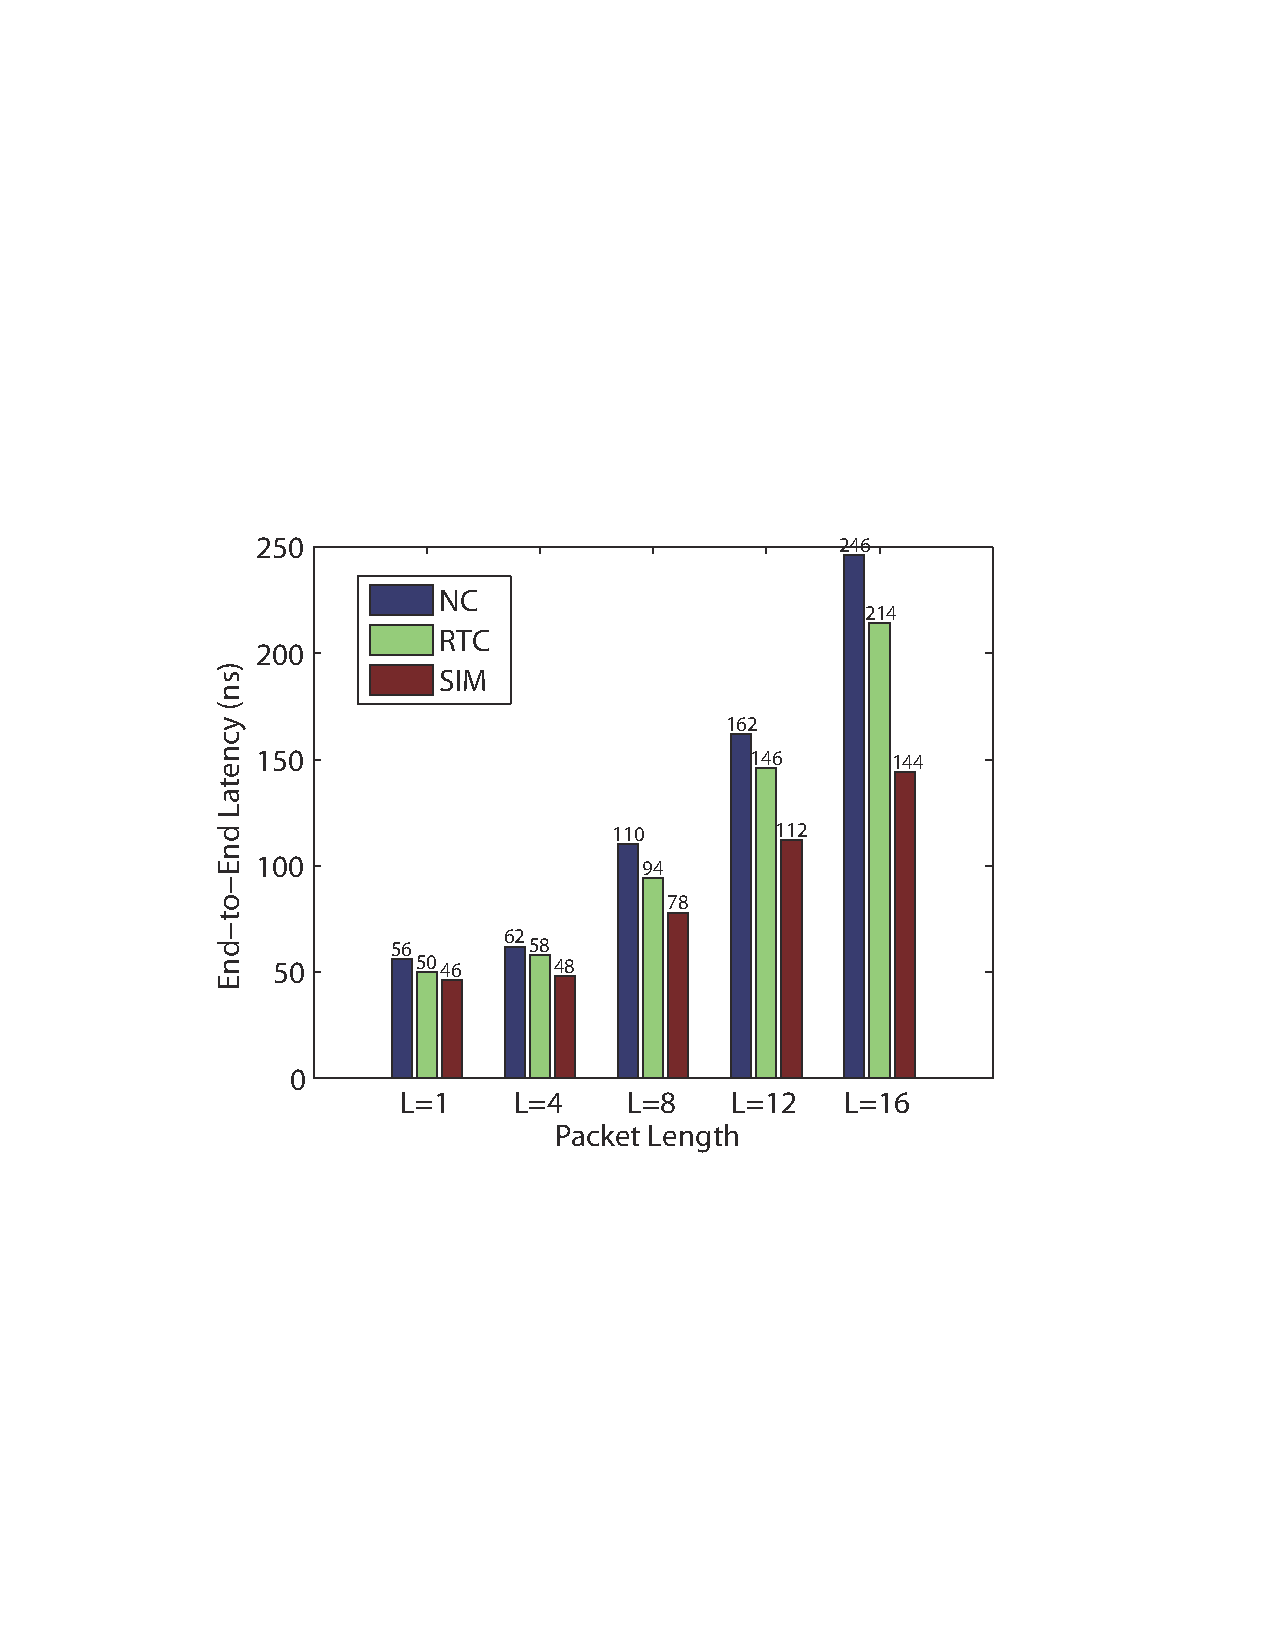
\includegraphics[scale=0.6]{figures/comparison.pdf}\\
  \caption{Comparison with network calculus and simulation}\label{comparison}
\end{figure}

Next, we explain the reason why our method outperform the DNC based method proposed in \cite{Qian489900}. As implied by Theorem 1.72 in \cite{Boudec2001Network}, if we can take the maximal service curve into consideration, we can get a much tighter output arrival curve, then, the leftover service curve of the next router will be much tighter than the one calculated with \cite{qian2009analysis}. To demonstrate this, let $B=4$, $L=4$ flits and $T=2ns$, we obtained the calculated service curve for flow $f_2$ both with DNC and RTC, as shown in Fig. \ref{loose}. The calculation was carried out with RTC toolbox. From Fig. \ref{loose}, we find that, the calculated service curve with RTC is much 'better' than DNC, which explains why the RTC can produce better results.
\begin{figure}
  \centering
  % Requires \usepackage{graphicx}
  \includegraphics[scale=0.6]{figures/loose.pdf}\\
  \caption{Comparison of service curve computed with real-time calculus and network calculus}\label{loose}
\end{figure}

\subsubsection{Buffer Optimization Comparison}
As has shown in previous subsections, the DNC based method \cite{Qian489900} can handle some circumstances that FLA and LLA can not be applied. This motivate us to optimize the buffer size of NoC with our method. Let the flit injection rate be $0.1$ flit/cycle, packet length $L=16$ flits and change the VC buffer depth from 4 flits to 10 flits, we compare the theoretical bound computed with DNC and our method, as shown in Fig. \ref{buffer}. It clear that, our method outperform the DNC based method, because it gives much tight bound for both $f_2$ and $f_3$. Further, if we set the deadline of $f_2$ and $f_3$ to 150ns, with our method, we can found that $B=8$ flits is sufficient enough to guarantee the delay bound. While the DNC based estimation is larger than $10$ flits. We also observed from Fig. \ref{buffer} that, the high priority flows (i.e. $f_1$ and $f_4$) are very insensitive to the buffer depths, which motivate us to allocate small buffers for these flows to reduce the area and power cost. Link-level analysis was extended in \cite{189} to finite buffer size scenario. But, we need to mention that, the LLA approach can not be applied to optimize the buffer size, this is because the network latency is larger than the injection period for this configuration.
\begin{figure*}
  \centering
  % Requires \usepackage{graphicx}
  \includegraphics[scale=0.5]{figures/buffer.pdf}\\
  \caption{End-to-end flows with different buffer size}\label{buffer}
\end{figure*}

We observed that, for the priority-aware NoC, the lower priorities, the higher blocking ratios, thus leading to larger buffer size.

\section{Conclusion}\label{conclusion}
The priority-aware wormhole-switched NoC is a promising platform for the on-chip real-time communication if the worst-case performance can be accurately analyzed and guaranteed. Simulation is not competent for this purpose because it is difficult to cover all the corner cases. In this paper, we propose an RTC based analytical model to achieve this goal. We first build the traffic model and service model for this NoC, and propose a novel method to derive the upper service curve of window flow control. Then, for the given task mapping and routing of each flow, we apply our RTC model to the follow two cases: (1) To verify whether all these flows meet their deadline under this configuration. We propose a latency analyzing algorithm to compute the end-to-end latency for each flow automatically. To improve the calculated delay bound, we proposed the concept of collapsible sub-path. (2) To optimize the buffer size of each router under the constraint of deadline. To achieve this goal, we propose an iterative algorithm to optimize the buffer from high priority flows to low priority flow gradually. Experiment results demonstrate that, our method outperforms the conventional scheduling theory and DNC based methods when the tightness of performance bound are considered. We also explain the rooted cause of this improvement. In addition, our results can also be applied to the mapping, routing and power optimization of NoC.

\section*{Acknowledgement}
The authors would thank the reviewers for their suggestions and comments, and all the experiments are carried out at Integrated Microsystem Lab (IML) of McGill University. This research is supported by High Technology Research and Development Program of China (Grant No. 2012AA012201, 2012AA011902).

\bibliographystyle{unsrt}
\bibliography{Docear}

\end{document} 